\chapter{Traceable Physics Models}
\label{chap:physics}

This thesis also contributes computational implementations of several key physics models for aircraft design that are traceable within the example code transformations framework introduced in Section \ref{sec:aerosandbox}, AeroSandbox. The broad motivation for this contribution stems from the observation that ``ease-of-model-implementation'' has historically proven to be one of the most important factors for determining whether an MDO paradigm can achieve use in industry. More specifically, the goals of this contribution are to:

\begin{enumerate}
    \item Stress-test the feasibility of code transformations in practice—how much added user effort and expertise is required to bring typical engineering analyses into a code-transformations-based MDO tool? To what extent can existing code be used as-is? Finally, the thesis aims to identify any specific computational elements that cause ``pain points'' when attempting to make an analysis traceable.
    \item Jump-start future applied research by providing a set of modular, plug-and-play analyses that can be used to quickly build a variety of aircraft design optimization problems. Since the long-term goal of this research direction is to establish whether the proposed MDO paradigm improves practicality, many practical aircraft design problems must be posed. Creating a set of modular general-purpose building blocks reduces the need to write similar analysis code repeatedly, saving time for designers.
\end{enumerate}

To achieve these goals, this thesis contributes the traceable implementations of the analyses given in Table \ref{tab:models_to_contribute}. This set of analyses was deliberately chosen to be mathematically diverse, spanning a wide range of common code patterns in scientific computing. The types of attributes that each analysis is intended to stress-test are given in the right-most column of Table \ref{tab:models_to_contribute}.

\begin{table}[H]

    \centering
    \caption{A list of aircraft design analyses that the thesis implements within a code transformations framework. The middle column lists the non-traceable tools for each analysis that are commonly used in industry today. The right-most column lists the computational attributes that each analysis is intended to stress-test.}
    \label{tab:models_to_contribute}
    \setstretch{1.25}
    \begin{tblr}{
        colspec={@{} X X X @{}},
        row{1}={font=\bfseries},
        hline{3-6}
    }
        \toprule
        Analysis To Contribute                            & Non-Traceable Analogue                                                        & Tests tracing through\ldots                                                                                                 \\ \midrule
        Vortex-Lattice Method Aerodynamics Analysis       & AVL \cite{avl}                                                                & An aerospace geometry engine and discretization; large, vectorized matrix methods, like linear solves                       \\
        Nonlinear Lifting Line Aerodynamics Analysis      & Phillips \& Snyder \cite{phillips_modern_2000}, Reid \cite{reid_general_2020} & Nonlinear systems of equations (i.e., implicit), which often lead to value-dependent code execution (via convergence loops) \\
        Workbook-style Aerodynamics Buildup               & USAF Digital DATCOM \cite{datcom}                                             & Table lookups, large amounts of conditional logic (yielding a wide, branching graph), and scalar-heavy math                 \\
        Rigid-Body Equations of Motion                    & ASWING (dynamics) \cite{aswing}                                               & Ordinary differential equations, which are often implemented in a loop-heavy way (yielding a deep graph)                    \\
        Linearized Aircraft Stability Modal Decomposition & AVL \cite{avl}                                                                & More advanced matrix methods, such as an eigenvalue decomposition                                                           \\
        \bottomrule
    \end{tblr}

\end{table}

These traceable implementations offer value within the context of the thesis itself (in stress-testing the practicality of code transformations), but they also have value as a standalone contribution to the aircraft design community—even outside of design optimization. Because of the mixed-backend numerics library described in Section \ref{sec:code_syntax}, these analyses can be used independently from the design optimization context of AeroSandbox if desired. In such cases, however, they still can retain certain runtime benefits from the code transformations framework, if desired by the user. For example, a traceable workbook-style aerodynamics buildup would seamlessly enable GPU-accelerated evaluations and automatic vectorization, offering significant speedups; an example application might be real-time performance estimation for model predictive controllers or flight simulation.


\section{Vortex-Lattice Method Aerodynamics Analysis}
\label{sec:vlm}

\subsection{Method Overview}
\label{sec:vlm_theory}

The vortex-lattice method (VLM) is a low-fidelity aerodynamics analysis used to model the inviscid 3D flow field around a system of lifting surfaces (e.g., wings). It is one of the most common conceptual-level aerodynamics analyses used in aircraft design, as it is computationally inexpensive and interpretable. Common tools that implement the VLM include AVL \cite{avl} and XFLR5 \cite{xflr5}.

A VLM analysis is based on classical potential-flow theory. Because this flow field model is a linear partial differential equation, it can be quickly solved using a boundary-element method representation by superimposing Green's-function kernels. These kernels model disturbances in the flow field that are induced by the lifting surfaces. In a VLM analysis, these kernels are modeled as a collection of \emph{horseshoe vortices} that are distributed along the wing in a regular lattice pattern (distributed in both spanwise and chordwise directions). A single horseshoe vortex is illustrated in Figure \ref{fig:horseshoe_vortex}. Each horseshoe vortex is a connected polyline of uniform-strength vortex filaments, with three segments: a bound vortex on the wing, and two trailing legs extending downstream to infinity\footnote{These trailing legs extend to the far-field Trefftz plane. In theory, these trailing legs should follow the local flow direction (and hence be ``force-free'' by the Kutta-Joukowski theorem), but often they are simply extended directly backwards which simplifies induced velocity computation and removes the need for an iterative wake relaxation.}. (In practice, a fourth leg consisting of a far-downstream ``starting vortex'' can be imagined to close the horseshoe vortex, which forms a ring vortex and thus satisfies the Helmholtz vortex theorems.) The Kutta condition is naturally satisfied, as the only place where the wing can shed vorticity is at the trailing edge (due to placement of the trailing legs).

\begin{figure}[h]
    \centering
    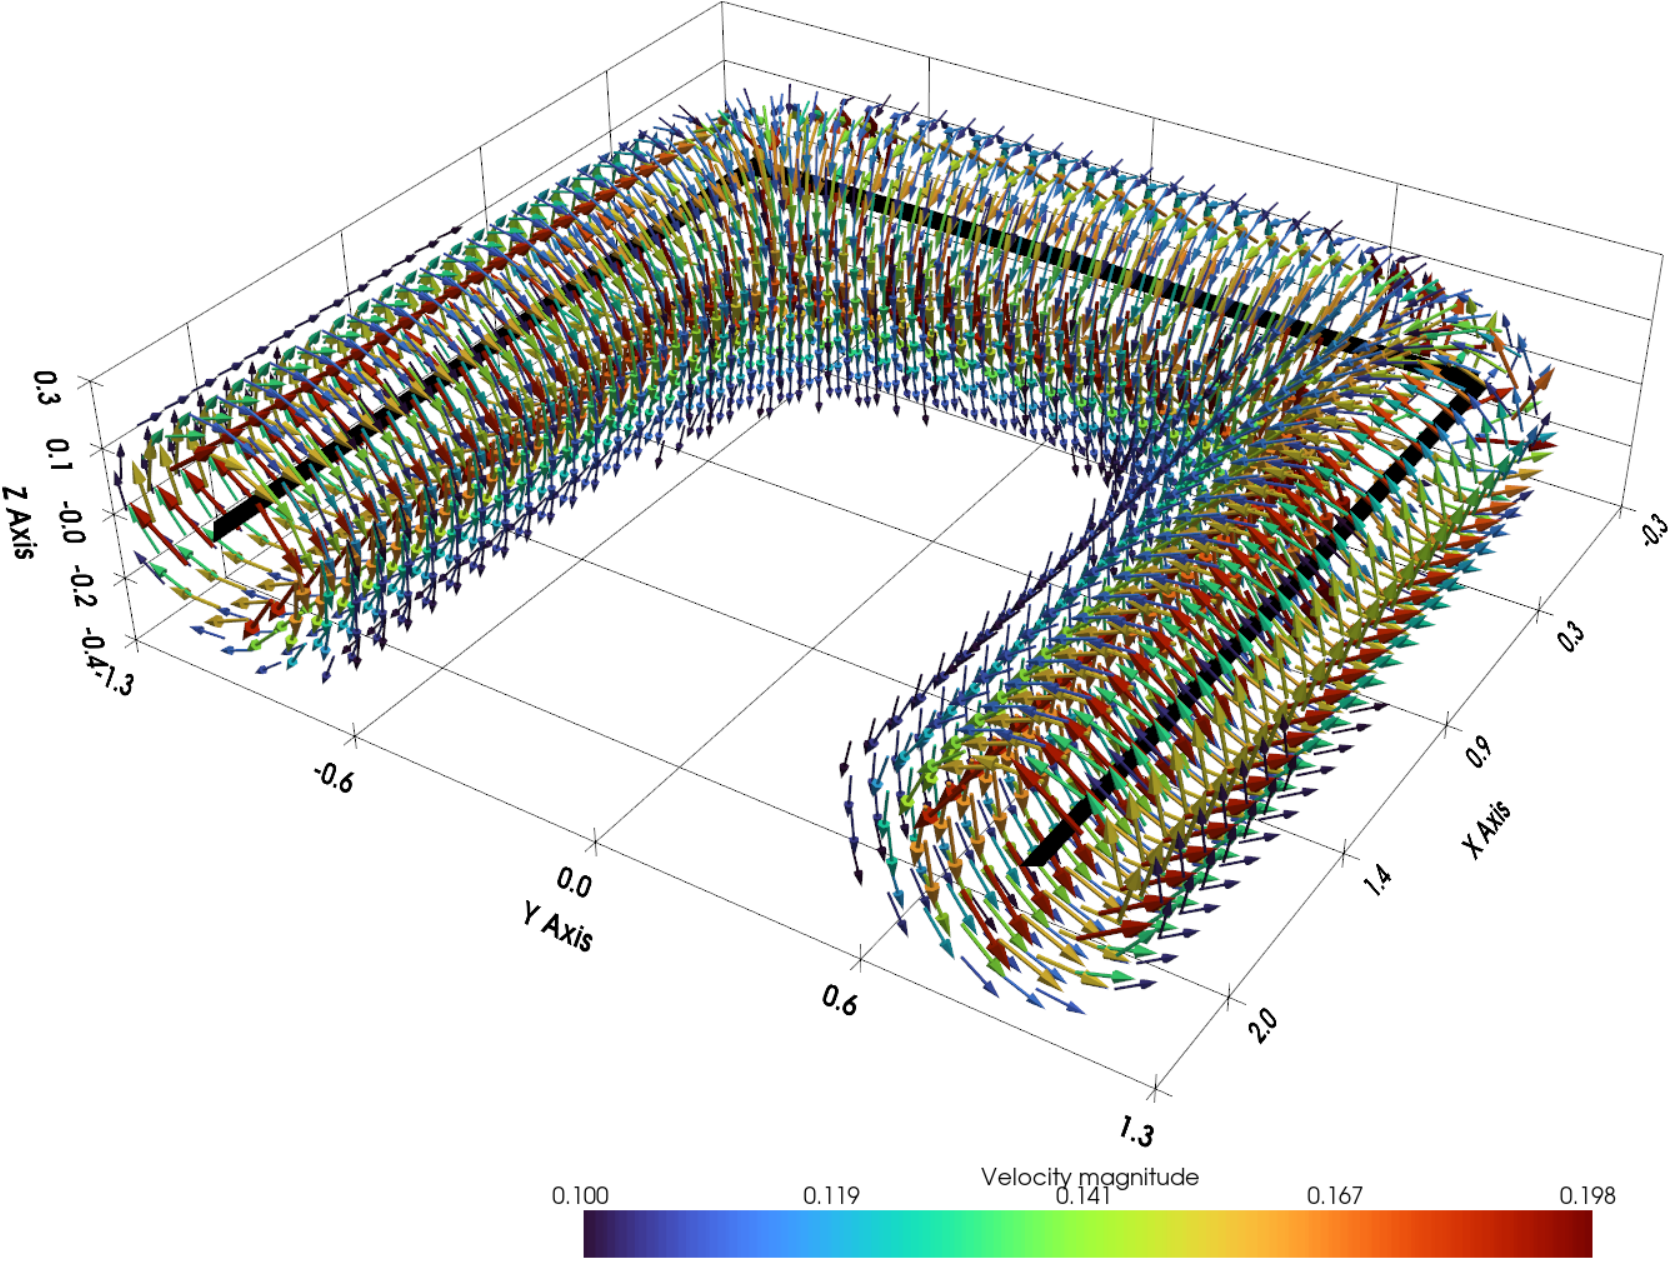
\includegraphics[width=5in]{../figures/horseshoe_vortex.png}
    \caption{Illustration of a horseshoe vortex (black) and the induced fluid velocity field around it, which is the fundamental building block of a VLM analysis. In reality the induced velocity field has global influence, but it is truncated here for conceptual clarity.}
    \label{fig:horseshoe_vortex}
\end{figure}


Each horseshoe vortex has an initially-unknown strength, and the vorticity associated with each vortex creates an induced velocity that affects the global flowfield. To solve for these $N$ unknown vortex strengths, $N$ constraints are needed. A convenient choice is to impose a \emph{flow-tangency} (also called \emph{no-penetration}) boundary condition associated with each horseshoe vortex, where the flow velocity normal to each horseshoe vortex is zero. It is not immediately obvious at which location this flow-tangency condition (called the \emph{collocation point}) should be imposed, relative to each horseshoe vortex. As it turns out, the best choice is to discretize the wing into quadrilateral panels, then place the bound leg at the quarter-chord point of each panel, and place the collocation point at the three-quarter-chord point. This choice results in higher-order convergence with respect to discretization resolution than any other choice, with derivation for this given by Katz and Plotkin \cite{katz_lowspeed_2004}. (One way to intuitively understand this reasoning is that the VLM is essentially a 3D analogue of 2D thin airfoil theory.)

Because of the linearity of the governing equations, the unknown horseshoe vortex strengths can be solved as a linear system of equations. Due to the global influence of each vortex on the flowfield, this linear system of equations is dense and asymmetric, so it is typically solved using LU factorization. The solution to this linear system gives the vortex strengths, which can then be used to reconstruct the flowfield around the lifting surfaces. The vortex strengths are also conveniently equal to the local difference in pressure coefficient between the top and bottom surfaces of the wing, which can be used to visually interpret the flow field. Lift force computation is usually performed using the Kutta-Joukowski theorem on each bound leg. Drag force calculation (which only includes induced drag, as a VLM is inviscid) can be accurately performed using a Trefftz plane wake integral. Further details on this analysis formulation are available in work by Katz and Plotkin \cite{katz_lowspeed_2004} and Drela \cite{drela_flight_2013}.

\subsection{Implementation}

\subsubsection{Discretization}

Based on this theory, a vortex lattice method was implemented into AeroSandbox as a traceable analysis. One of tasks when implementing this analysis is discretizing the geometry (i.e., generate a mesh) in a code-transformations compatible way. Because discretization of a high-level geometry representation is such a common task in engineering analysis, an aircraft geometry stack was built within AeroSandbox to facilitate this. This stack allows one to represent an aircraft geometry at a conceptual level (i.e., within a hierarchical data structure that is not tied to any specific analysis), and then to generate a variety of degenerate geometry representations from this conceptual geometry. These degenerate geometry representations could be a series of 1D beams (for structural analysis), a mean camber line geometry representation (for a VLM aerodynamics analysis), a 3D panel geometry representation (for visualization or for CFD analysis), or any other representation that is needed for a specific analysis. Examples of such degenerate geometry representations that are possible are illustrated in Figure \ref{fig:degen_geometry}. This capability to separate the concept of geometry from its representation makes it much easier to implement multi-physics analysis that may be required in MDO problems.

Conceptually, the ideas behind this geometry stack are inspired by the degenerate geometry representation capabilities of OpenVSP \cite{mcdonald_open_2022}, with the difference that this is built on top of a traceable numerics core. Because of this, these meshes gain all the properties enabled by code transformations, such as differentiable meshing. Furthermore, if analyses are built on top of this geometry stack, the analysis can be end-to-end differentiable throughout both discretization and solution.

This unified, vertically-integrated workflow contrasts with many current design optimization workflows, which instead usually treat meshing and solving as separate black-box tools. In cases where end-to-end gradients are required (i.e., aerodynamic shape optimization with respect to a set of design variables), the usual strategy is to compute gradients for each process and then later to stitch them together. For example, a meshing tool might use forward-mode automatic differentiation\footnote{or, if the mesh has a deterministic connectivity (i.e., hyperbolic marching from a surface), one could use a method with similar properties, like complex-step differentiation or finite-differencing}, while a solver might use a discrete adjoint of the governing PDE to obtain mesh gradients. Stitching these gradients together is a perfectly viable solution from a computational perspective, but as a practical matter it often requires a fair amount of boilerplate code from the user. In contrast, unifying the meshing and solution processes within a code transformations framework eliminates the need for the user to manually interact with component partials, lessening the expertise required to build a differentiable analysis.

\begin{figure}[h]
    \centering
    \begin{subfigure}{0.32\textwidth}
        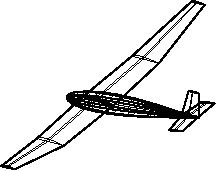
\includegraphics[width=\textwidth]{../figures/geometry_concept-crop.pdf}
        \caption{Concept-level geometry representation, corresponding to the raw data structures within the AeroSandbox geometry stack.}
        \label{fig:geometry_concept}
    \end{subfigure}
    \begin{subfigure}{0.32\textwidth}
        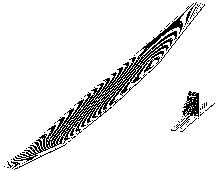
\includegraphics[width=\textwidth]{../figures/geometry_mean_camber-crop.pdf}
        \caption{Mean camber line degenerate geometry representation, which is used during VLM analysis.}
        \label{fig:geometry_mean_camber}
    \end{subfigure}
    \begin{subfigure}{0.32\textwidth}
        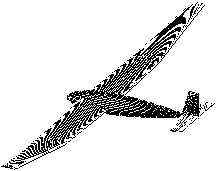
\includegraphics[width=\textwidth]{../figures/geometry_panel-crop.pdf}
        \caption{3D panel degenerate geometry representation, which can be used in other aerodynamic analyses.}
        \label{fig:geometry_panel}
    \end{subfigure}
    \caption{Illustration of several possible degenerate geometry representations produced by the AeroSandbox geometry stack. This removes the need for individual disciplinary analyses to re-implement their own meshing tools, creating a clearer API for new analysis tool development.}
    \label{fig:degen_geometry}
\end{figure}

\subsubsection{Solution Methodology Considerations}

With meshing complete, the governing system of equations described in Section \ref{sec:vlm_theory} can be implemented. Within the context of a code transformations framework, an interesting question is whether this system should be solved explicitly or implicitly. To clarify the difference here:

\begin{itemize}
    \item In an \textbf{explicit} formulation, the matrix and right-hand-side vector of the linear system of equations are explicitly constructed within the analysis code, and the system is solved using a direct solver. In the context of a broader optimization problem encompassing such a model, this means that a) the system of governing equations is solved exactly at each iteration, and b) no optimization variables or constraints are added to the solve.

    \item In an \textbf{implicit} formulation, the horseshoe vortex strengths are posed as optimization variables, and the governing equations are implemented in residual form and constrained (in the top-level optimzation problem) to be driven to zero. This is analogous to a simultaneous-analysis-and-design MDO problem formulation (shown in Figure \ref{fig:sand}). Here, the matrix and right-hand-side vector of the linear system are never explicitly constructed within the analysis code (though of course, the optimization problem constraint Jacobian will essentially compute this same information). In the context of a broader optimization problem encompassing such a model, this means that a) the system of governing equations is solved approximately at each iteration, and b) optimization variables and constraints are added to the solve.

\end{itemize}

Both methods have advantages. The principal advantage of the explicit formulation is that incorporating this into a design optimization framework can yield more stable convergence, since ``correct'' (i.e., zero-residual) solutions are guaranteed at each iteration. This can be especially important in the context of a multidisciplinary optimization problem, where this VLM analysis might be combined with other analyses. Here, a fully coupled implicit system might become numerically unstable (e.g., numerically-stiff), leading to convergence difficulties.

On the other hand, the implicit formulation has the potential to be much faster, in the context of a broader optimization problem. This is because the optimizer is solving for primal feasibility (i.e., constraint violation) and dual feasibility (i.e., optimality conditions) simultaneously. An intuitive way to think about this is that the optimizer is not wasting CPU cycles by solving the analysis accurately during early iterations, when the solution is far from the optimum. Instead, the optimizer is solving the analysis just enough to ensure that the constraints are satisfied, and then moving on to the next iteration. This can lead to significant speedups (up to an order of magnitude, in the author's experience) in the context of a broader optimization problem, especially when the analysis is expensive to solve.

There are also some cases where this implicit solution can be favorable in augmented analyses. For example, if a panel method is coupled with an integral boundary layer model (e.g., in XFoil), solving the problem as a coupled system rather than a segregated disciplinary solve can resolve singularity issues that might otherwise appear \cite{drela_xfoil_1989, drela_viscousinviscid_1987, ranneberg_viiflow_2019, fidkowski_coupled_2022, zhang_threedimensional_2022}.

In the case of the present VLM implementation, both formulations are offered, with the explicit solution being the default. This is because the explicit solution is more stable and easier to debug, and because the VLM analysis is relatively inexpensive to solve. However, the implicit solution is also available, and can be used if the user desires faster convergence in the context of a broader optimization problem.

\subsection{Example Results}

Figure \ref{fig:vlm} shows the results of a VLM analysis performed using AeroSandbox, using a generic glider design and a prescribed aerodynamic operating point. At the moderately high paneling resolution shown here ($N=700$ panels), solution takes about 0.25 seconds on a laptop-grade CPU. The surface color shows the vortex strength (or equivalently, $\Delta C_p$ across the wing), while the streamlines show the flow field.

\begin{figure}[h]
    \centering
    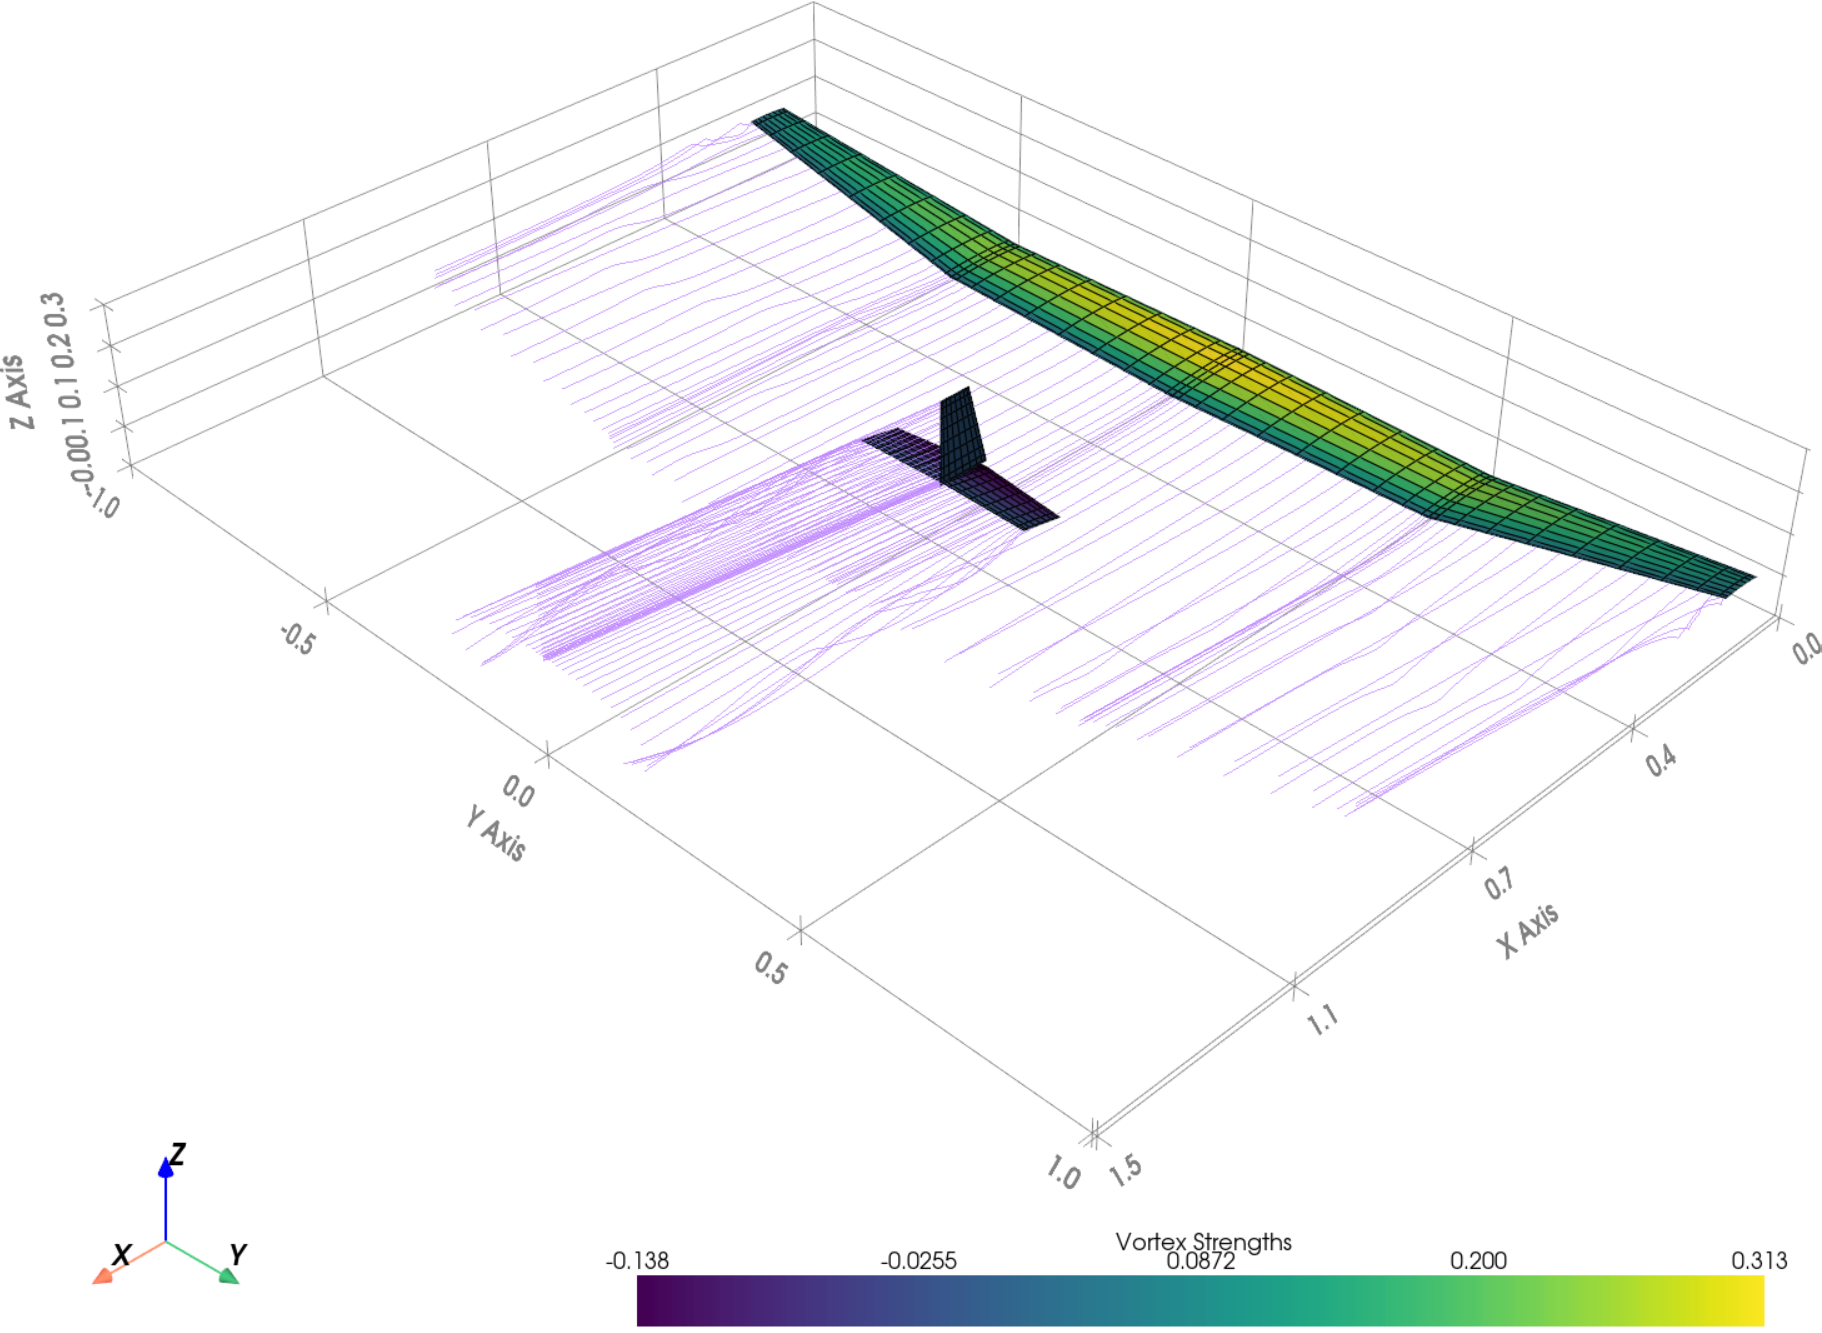
\includegraphics[width=\textwidth]{../figures/vlm.png}
    \caption{AeroSandbox VLM analysis results for a simple glider geometry at a prescribed aerodynamic operating point. Surface color shows the vortex strength (or equivalently, $\Delta C_p$ across the wing). Streamlines show the flow field.}
    \label{fig:vlm}
\end{figure}

Quantitative validation results for this VLM analysis are shown later in Section \ref{sec:aero_validation}, where the VLM can be cross-compared not only against external tools but also against the other plug-and-play aerodynamic analyses developed in this chapter. Notably, while the VLM method is quite accurate for computing induced drag, it has no mechanism to compute profile drag without augmentation by another aerodynamic method, like the buildup described in Section \ref{sec:aerobuildup}; hence, the VLM method should not be used by itself for performance analysis. It is, however, more than adequate for flight dynamics analysis, as there are few other low-fidelity aerodynamics methods that handle local velocity effects (e.g., dynamic derivatives, aerodynamic damping) as accurately.

\subsection{Aerodynamic Shape Optimization}

To demonstrate how this VLM tool can be incorporated into a broader optimization problem, we can formulate a classic aerodynamic shape optimization problem and compare our result to a known solution.

Here, we aim to find the minimum-induced-drag wing planform, by optimizing a wing's chord distribution. We assume:

\begin{itemize}[noitemsep]
    \item A fixed total lift
    \item A fixed wing area
    \item A fixed span
    \item An untwisted, uncambered, unswept, thin, planar wing
    \item Potential flow (inviscid, incompressible, irrotational, and steady)
\end{itemize}

For this fixed-span, fixed-lift case, theory shows that the minimum-induced-drag wing has an elliptical lift distribution. With the additional assumptions above, the corresponding minimum-induced-drag wing will also have an elliptical \emph{chord} distribution \cite{anderson_fundamentals_2009}.

This problem can be posed in AeroSandbox syntax using the plug-and-play VLM analysis model described in the previous section. We supply an initial guess of a simple rectangular (i.e. untapered) wing, and optimize the chord distribution. We do not know the correct angle of attack $\alpha$ to achieve our specified lift coefficient \emph{a priori}, so this becomes an additional optimization variable. The VLM is implemented, here using just one spanwise panel for each unknown chord variable—typically, a higher resolution ($\sim 4$ panels per optimization variable) would be used for numerical stability, but this is used to demonstrate numerical robustness of the implementation here.

Surprisingly, the entire optimization problem can be written in less than 40 lines of code, allowing it to be shown in its entirety in Listing \ref{lst:vlm_optimization}. This serves as a good illustration of the motivation behind developing these plug-and-play models for a code transformations framework—the modularity allows complex optimization problems to be posed with minimal code.

\begin{listing}[H]
    \begin{minted}{python}
import aerosandbox as asb
import aerosandbox.numpy as np

opti = asb.Opti()  # Initialize an optimization environment.

N = 16  # Spanwise resolution
y = np.sinspace(0, 1, N, reverse_spacing=True)  # Spanwise locations along the wing.
chords = opti.variable(init_guess=1 / 8, n_vars=N, lower_bound=0)  # Chord dist.
wing = asb.Wing(  # Defines the wing geometry.
    symmetric=True,
    xsecs=[  # Cross sections ("XSecs") of the wing
        asb.WingXSec(
            xyz_le=[  # Location of each cross-section's leading edge
                -0.25 * chords[i],  # This keeps the quarter-chord-line straight.
                y[i],  # Our (known) span locations for each section.
                0
            ],
            chord=chords[i],
        )
        for i in range(N)
    ]
)

aero = asb.VortexLatticeMethod(  # Compute aerodynamics using the VLM analysis
    airplane=asb.Airplane(wings=[wing]),  # The geometry to analyze
    op_point=asb.OperatingPoint(  # Aerodynamic operating condition
        velocity=1,  # A fixed velocity; unimportant due to nondimensionalization.
        alpha=opti.variable(init_guess=5, lower_bound=0, upper_bound=30)  # Angle of attack
    ),
    spanwise_resolution=1,  # Uses one panel per wing cross-section
).run()

opti.subject_to([
    aero["CL"] == 1,  # We want a fixed lift coefficient
    wing.area() == 0.25,  # We want a fixed wing area
])

opti.minimize(aero["CD"])
sol = opti.solve()
    \end{minted}
    \caption{AeroSandbox code to optimize the chord distribution of a wing to minimize induced drag.}
    \label{lst:vlm_optimization}
\end{listing}

The optimization problem is solved to tolerance within 18 IPOPT iterations, corresponding to around 10 seconds of wall-clock time on a laptop CPU. This yields the wing geometry shown in Figure \ref{fig:vlm_opt}, which is indeed elliptical in chord distribution. To confirm, the chord distribution can be directly compared to an elliptical distribution as shown in Figure \ref{fig:vlm_opt_compare}. Very slight differences appear due to numerical discretization, but as panel resolution is increased, these results converge.

\begin{figure}[h]
    \centering
    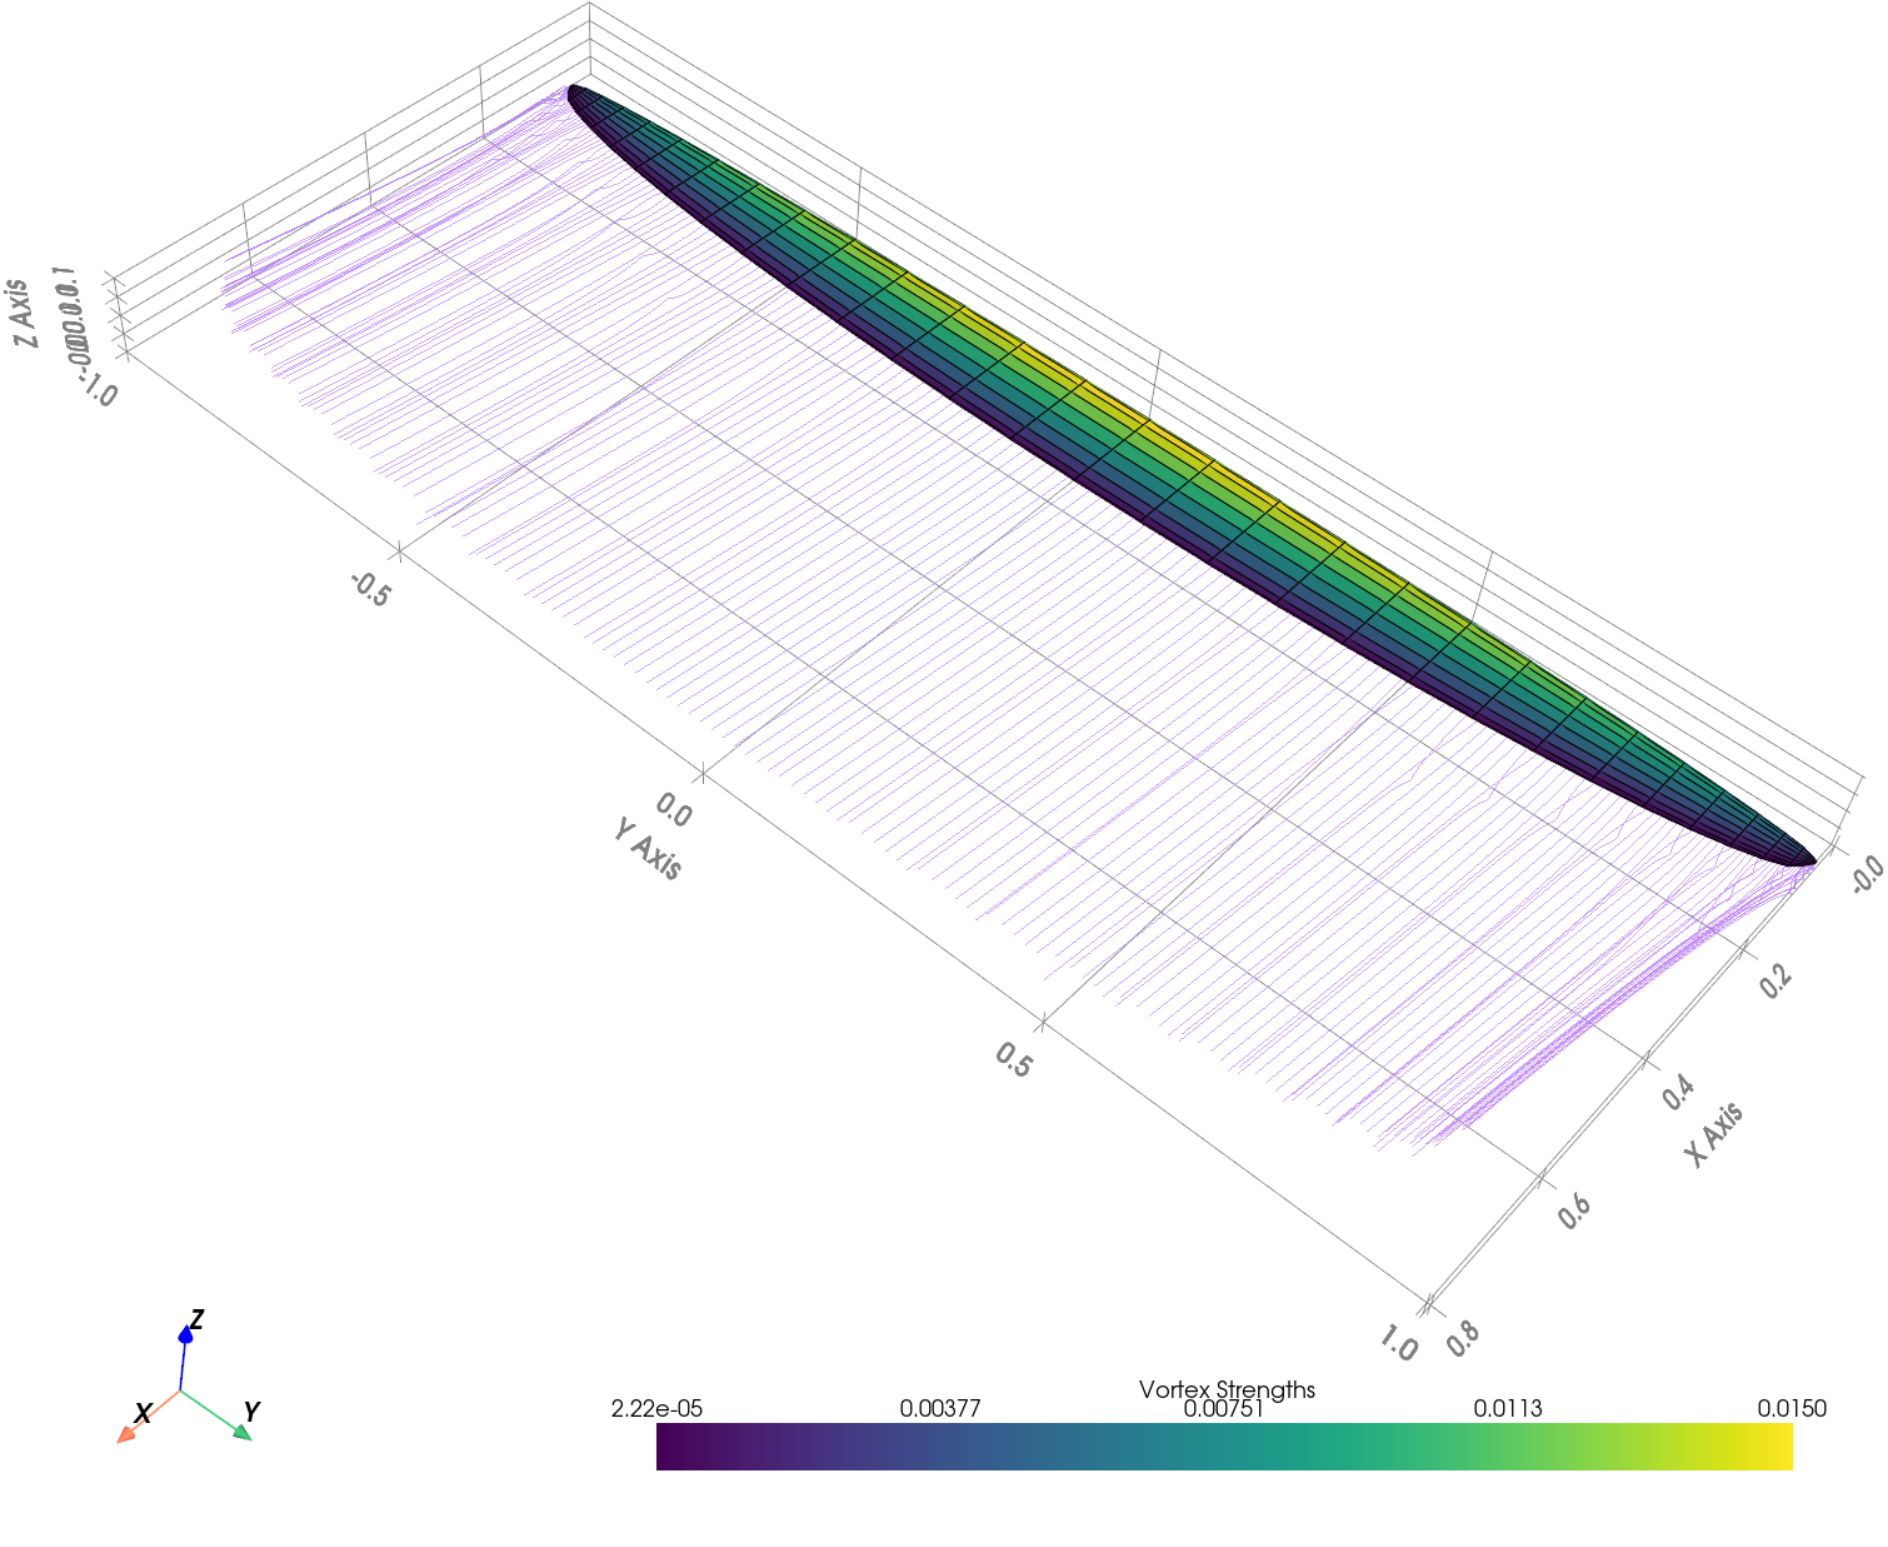
\includegraphics[width=\textwidth]{../figures/vlm_opt.png}
    \caption{Result of the AeroSandbox VLM analysis-based aerodynamic shape optimization problem. The optimized wing has an elliptical chord distribution.}
    \label{fig:vlm_opt}
\end{figure}

\begin{figure}[h]
    \centering
    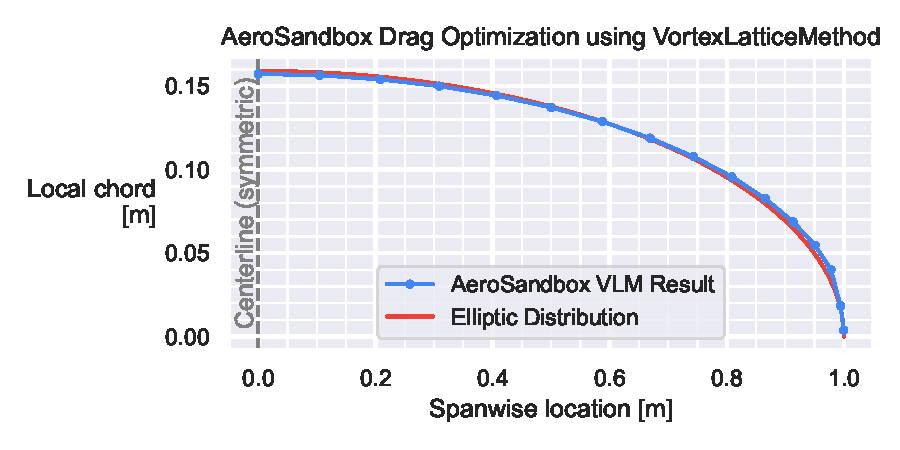
\includegraphics[width=\textwidth]{../figures/vlm_opt_compare.pdf}
    \caption{Comparison of the optimized chord distribution to the theoretical elliptical chord distribution.}
    \label{fig:vlm_opt_compare}
\end{figure}

\section{Nonlinear Lifting Line Aerodynamics Analysis}
\label{sec:ll}

\subsection{Method Overview}

While the VLM described in Section \ref{sec:vlm} is a useful tool in conceptual analysis, its inviscid nature means that it cannot capture many important aerodynamic effects. This includes profile drag effects, but also more subtle effects like nonlinear sectional lift curve slopes and local stall. Another downside of the VLM is that capturing camber effects requires a substantial number of chordwise panels, which quickly increases the size of the linear system\footnote{The solve time of this linear system scales as $\order(N^3)$ with the number of panels, so keeping the number of panels low is quite valuable.} without meaningfully improving the induced drag prediction (as this is dominated by spanwise effects).

One way to address both of these limitations is to use a lifting-line method instead of a VLM. A modern lifting-line method is best conceptually understood as a vortex lattice method with several key similarities and differences:
\begin{enumerate}
    \item First, just as with the VLM, the lifting-line method uses a potential flow model with horseshoe vortices to model the flow changes induced by the vehicle.
    \item Another difference is that in a lifting-line method the governing equation no longer comes from a flow-tangency condition. Instead, the constraint relationship comes from equating the lift force generated by the vortex (via the Kutta-Joukowski theorem) to the lift force computed using a 2D sectional model (i.e., airfoil-level data) and the local angle of attack.
    \item A notable difference is that in a lifting line method only one chordwise panel is required, because camber effects are not captured by direct flow tangency over the curved surface.
\end{enumerate}

This constraint relationship, which is detailed further in by Phillips and Snyder \cite{phillips_modern_2000}, allows the lifting-line method to leverage the accuracy of 2D sectional data, which can include camber effects. In almost all existing lifting-line methods, the sectional data is approximated using an affine $C_L$-$\alpha$ relationship (possibly with a nonzero $C_L$ at $\alpha=0$ to capture camber effects), because this reduces the governing system of equations to a single linear solve (just as with the VLM). This is computationally faster to solve than the true nonlinear problem. However, this also loses substantial accuracy in lift prediction, especially in cases where nonlinearities in the lift curve are important, such as near transitional Reynolds numbers and in high-lift cases. In many cases, this may make the traditional linear lifting-line method unsuitable.

Because of this, the present work implements \emph{both} a linear and nonlinear lifting line method, with the latter retaining the full (nonlinear) lift curve slope behavior. This is done by reformulating the method to be implicit, with governing equations converted into nonlinear residual form.

In both the linear and nonlinear methods, 2D sectional data is provided using \emph{NeuralFoil}, a custom physics-informed machine learning method described in Chapter \ref{chap:physics-informed-ml}. Using NeuralFoil to obtain sectional data has negligible error compared to XFoil solutions, and it has the important property of retaining $C^1$-continuity that allows for gradient-based rootfinding methods to be used in the nonlinear case. With the linear method, the NeuralFoil evaluation is numerically differentiated about the geometric angle of attack of each wing cross section\footnote{In other words, the angle of attack with respect to the freestream velocity vector (which can be computed explicitly), not the local perturbed fluid velocity vector (which is an implicit function of the initially-unknown vortex strengths)} to construct an affine $C_L(\alpha)$ dependency. Critically, because of this local linearization step about the geometric angle of attack, even the linear lifting-line method in the implementation here can capture limited stall effects—this is a unique feature of the present work compared to other lifting-line implementations.

%The nonlinear lifting-line method has one notable drawback, which is that unlike a linear lifting-line, it is not guaranteed to produce a solution. This mostly occurs  inversion of the $C_L(\alpha)$ curve, which occur

The overall lifting line methodology presented in this section represents modern thinking about the theoretical formulation of lifting-line methods, as given by Phillips and Snyder \cite{phillips_modern_2000} and Reid \cite{reid_general_2020}; this is a generalization of the historical lifting-line formulation originally given by Prandtl in the early 20th century. The general formulation presented here has been shown to work well for non-straight lifting lines, which occurs in wings with sweep or dihedral \cite{reid_general_2020, jacobs_extension_2012, phillips_liftingline_, phillips_modern_2000}.

\subsection{Implementation}

%The lifting-line method was implemented in AeroSandbox as a traceable analysis. Both the linear and nonlinear lifting lines are

The linear version is implemented similarly to the VLM implementation, where both an explicit and an implicit solve are possible. On the other hand, the fully nonlinear lifting-line method is currently only implemented as an implicit analysis.

Numerical discretization is performed by thin-surface meshing with a chordwise paneling resolution of one. The quarter-chord lines of these panels can then be connected to obtain a lifting line for the wing.

\subsection{Example Results}

Figure \ref{fig:ll} shows analogous lifting-line analysis results for the same glider example as the VLM analysis. The reduction in discretization resolution due to the elimination of chordwise refinement is immediately apparent from the lower number of discrete panels. This leads to much shorter asymptotic runtimes, especially for vehicles with complex systems of multiple interacting lifting surfaces.

\begin{figure}[h]
    \centering
    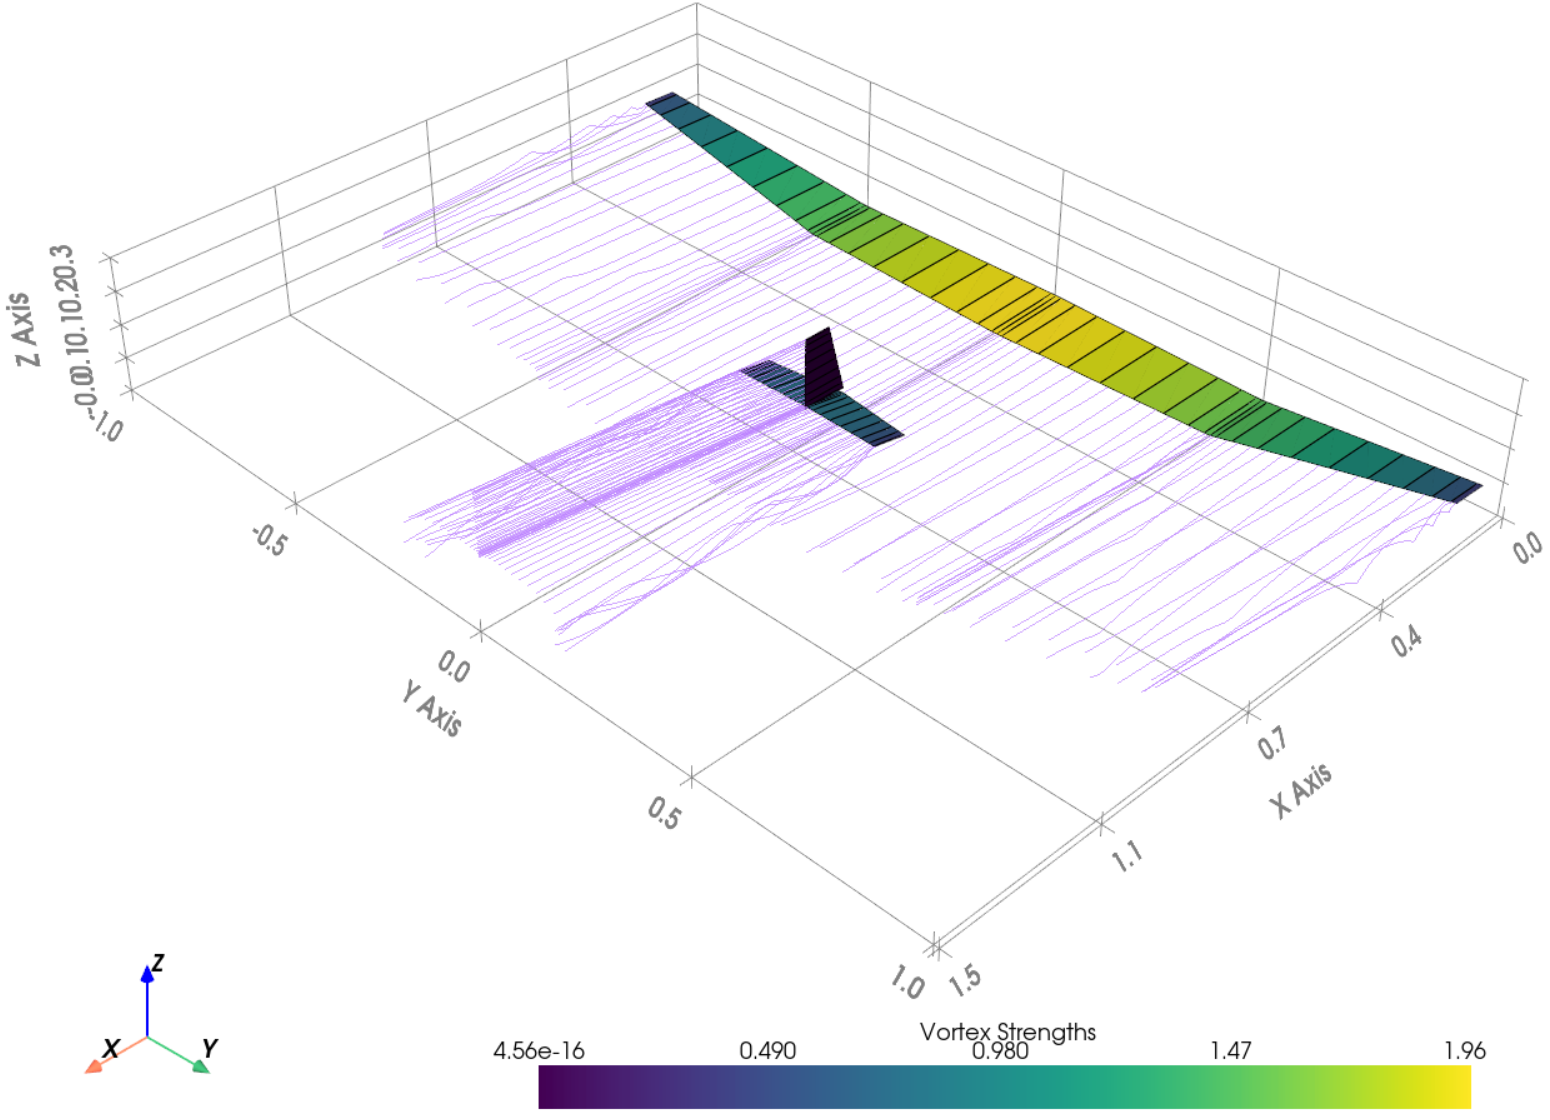
\includegraphics[width=\textwidth]{../figures/ll.png}
    \caption{AeroSandbox lifting-line analysis results for a simple glider geometry at a prescribed aerodynamic operating point. Surface color shows the vortex strength (or equivalently, $\Delta C_p$ across the wing). Streamlines show the flow field.}
    \label{fig:ll}
\end{figure}

As with the VLM, quantitative validation results for this lifting-line analysis are shown later in Section \ref{sec:aero_validation}. In general, the lifting-line method is expected to be more accurate than the VLM for aerodynamic performance prediction purposes (i.e., lift, drag, and moment prediction), due of the incorporation of 2D sectional data. The lifting line also generally leads to more interpretable results, as the local angle of attack, lift coefficient, downwash, and other properties of interest can be directly returned by the analysis. (In a VLM, these quantities must be obtained by integration along the chord, which introduces error and creates extra postprocessing work depending on the data structure of the mesh.)

On the other hand, the VLM has advantages in low-aspect-ratio cases (as spanwise flow becomes more significant, invalidating the force-free wake assumption on the straight trailing vortices), in other highly-3D flow fields, and for angular rate stability derivatives (as the VLM can better capture chord-wise variations in local velocity).

\section{AeroBuildup: A Workbook-style Aerodynamics Buildup}
\label{sec:ab}

\begin{attrib}
    This section includes content from the author's contributions to the AeroSandbox documentation \cite{asb_github}.
\end{attrib}

\subsection{Method Overview and Implementation}

While the VLM and lifting-line methods in Sections \ref{sec:vlm} and \ref{sec:ll} provide conceptual-level aerodynamics analyses with strong first-principles grounding, they are limited in their ability to capture many important aerodynamic effects. For example, compressibility effects, fuselage aerodynamics, and high-angle-of-attack aerodynamics all go beyond the capabilities of these methods. Furthermore, these methods can have scalability challenges in combined-vehicle-and-trajectory optimization problems, depending on problem formulation. For example, the Firefly design problem of Section \ref{sec:firefly} requires aerodynamic solutions to be computed at \emph{each} of 200 unique points along the flight trajectory, at each iteration. Computing these solutions using a VLM or lifting-line method\footnote{The astute reader will notice that, in the case of a linear method where geometry and aerodynamic operating point can be separated (like the VLM), one possible strategy to improve this scaling is by saving the LU-factorization and back-substituting unique right-hand-side vectors. However, no analogous strategy exists if either the method is fully nonlinear or if the coefficient matrix depends on the operating point, as is the case with the lifting line implementation here.} increases the total optimization runtime to the point where real-time interactive design is no longer attractive (i.e., an hour or longer), limiting the tool's utility in gathering conceptual design intuition.

To address these problems and provide a practical alternative, AeroSandbox includes a rapid, vectorized aerodynamics engine called AeroBuildup. AeroBuildup's methodology essentially uses a workbook-style buildup to compute aerodynamic forces, moments, and (optionally) stability derivatives. It attempts to model viscous and compressible effects on wings and fuselages across any orientation (360 degrees of $\alpha, \beta$) and arbitrary vehicle angular rates ($p$, $q$, $r$). Just as with the VLM and lifting-line methods, the input is both the vehicle geometry\footnote{The vehicle geometry includes a reference point, which is used for moments and stability derivatives.} and an aerodynamic operating point\footnote{An operating point consists of the local atmospheric conditions, airspeed, orientation (angle of attack $\alpha$ and sideslip angle $\beta$), and angular rates ($p$, $q$, and $r$ about the three principal aircraft body axes).}.

AeroBuildup combines a variety of both theoretical and empirical models, inspired heavily by the methodology used by USAF Digital DATCOM \cite{datcom}. (Indeed, many of the submodels are directly shared with Digital DATCOM.) Compared to DATCOM, however, AeroBuildup has several advantages that make it more favorable as an analysis to use within a larger aircraft design optimization problem:

\begin{enumerate}
    \item AeroBuildup aims to \emph{smoothly} model across a wide variety of flight regimes; the model returns $C^1$-continuous aerodynamic results that span from subsonic to supersonic speeds, from attached to separated flow, and from the lowest to highest Reynolds numbers. This contrasts with DATCOM, which requires the user to select submodels appropriate to the flight regime (e.g., small-scale transonic flight), and produces discontinuous results in some cases (e.g., as soon as Mach number crosses a threshold, DATCOM instantly switches to a different wave drag model, which causes a discontinuity in the drag prediction).

    \item AeroBuildup makes minimal assumptions about the vehicle configuration. For example, with AeroBuildup any number of wings and fuselages may be specified, and these may be placed in any location; DATCOM forbids certain configurations, such as those with multiple fuselages. As another example, all lifting surfaces in AeroBuildup are simply ``Wing'' objects--the user isn't required to provide any extra semantic meaning (i.e., whether a surface is a horizontal vs. vertical stabilizer) that would change physics modeling. This contrasts with DATCOM, which requires explicit labeling. The end result is that AeroBuildup enables optimization with respect to parameters that are simply not possible with DATCOM\footnote{For example, imagine an airplane with a V-tail, where we wish to optimize the V-tail dihedral angle. DATCOM requires this to be entered as either a horizontal or vertical stabilizer, but it is not clear at what V-tail dihedral angle that switch should be made. This distinction changes DATCOM's results, but of course in reality the actual flow physics should not depend on the semantic label that we give it.}.

    \item AeroBuildup is end-to-end vectorized, which means that multiple aerodynamic operating points can be analyzed simultaneously with hardware-level (SIMD) parallelism. This is especially advantageous in a semi-empirical model like AeroBuildup, as many of the submodels consist of scalar-heavy analytical equations where vectorization buys significant speedups. Because of this vectorization, AeroBuildup is fast enough to be used in combined-vehicle-and-trajectory optimization problems, as demonstrated in Sections \ref{sec:firefly} and \ref{sec:dawn}.

    \item AeroBuildup is designed to be hackable, which allows end-users to easily tweak the analysis for problem-specific considerations without requiring a bespoke aerodynamics analysis. This is facilitated by a) implementation in an accessible high-level language, Python, and b) a codebase that is modular and hierarchical.

    \item AeroBuildup is implemented in an accessible high-level language, Python, which makes it easier for end-users to modify or extend the analysis with problem-specific considerations. The AeroBuildup codebase is also modular and hierarchical; this isolation of components limits the scope that a new user must understand to make a modification.

\end{enumerate}

The basic philosophy of AeroBuildup's approach revolves around a) hierarchical decomposition of the vehicle geometry, b) modeling of individual pieces, and then c) corrections for interactional effects between those pieces. For example, AeroBuildup computes aerodynamics on a per-wing and per-fuselage level, and further breaks down each of these into sectional aerodynamics.

For each wing section, the freestream velocity is computed in the local frame, with streamwise, normal, and crossflow velocities. A rotation-induced local flow velocity is also added to this, which later enables downstream computation of dynamic stability derivatives. This approximate local flow information is used to compute a set of \emph{tentative} sectional aerodynamics (including viscous and compressible effects) using NeuralFoil, a physics-informed machine learning model described in Chapter \ref{chap:physics-informed-ml}. These tentative sectional aerodynamics are then corrected for the wing's self-induced downwash, for 3D compressible effects, and for other 3D effects (e.g., the unsweeping of a lifting line near the root of a swept wing). Induced drag is computed by assuming the wake flows back to the Trefftz plane by projecting the wing's lifting line in the direction of the freestream velocity. After these corrections, the sectional aerodynamics are integrated along the span to obtain the total aerodynamic forces and moments.

Currently, a notable omission of the AeroBuildup model is the influence of downwash from \emph{other} wings; this has the benefit of improving computational speed, but it can lead to inaccuracies in the presence of strong interactions between lifting surfaces. (For example, when analyzing a conventional-configuration airplane using AeroBuildup, the effectiveness of the horizontal stabilizer will usually be slightly overestimated due to the missing downwash influence of the main wing\footnote{One way to conceptually think about this is that the effective lift-curve-slope of the horizontal stabilizer, $C_{L\alpha, h}$, should be slightly reduced due to main-wing downwash; this effect is not captured.}.)

Fuselage modeling generally follows methods described by Jorgensen \cite{jorgensen_method_1973, jorgensen_prediction_1979} and MIL-HDBK-762 \cite{_design_1990}. More precisely, inviscid results are theoretically grounded in slender body theory \cite{fva}, while viscous effects are modeled using an infinite-length crossflow analogy with finite-length corrections. The AeroSandbox geometry stack admits both circular and non-circular fuselages \footnote{Precisely, fuselage cross sections may be superellipse curves with any positive value of the shape parameter.}, and the dependence of crossflow separation location on local fuselage curvature (i.e., corners) is modeled. Wake separation, base drag, and any associated extra lift generation is handled using empirical methods fitted to wind tunnel results on a series of typical body shapes. Likewise, local velocity overspeed and any associated wave drag in transonic cases is computed using empirical relations.

AeroBuildup is a fully explicit calculation method, which means that a result is guaranteed in bounded computational time, without any non-convergence issues. However, the accuracy of this result is strongly dependent on the flight regime of the case in question. For example, AeroBuildup is expected to be most accurate for typical flight conditions where theory is sound and experimental data for validation sub-models is widely available. Generally, this well-behaved region includes flows without regions of massive separation or strong shocks. (AeroBuildup also remains relatively accurate in cases with low and transitional Reynolds numbers, due to viscous methods described in Chapter \ref{sec:physics-informed-ml}.) Quantitative validation results for AeroBuildup against other methods are shown later in Section \ref{sec:aero_validation}.

On the other hand, cases at extreme flight conditions (e.g., $\alpha=90\degree$, $\M_\infty=1.00$) will be much less accurate. However, even in these cases, effort has been taken such that the results from AeroBuildup are at least order-of-magnitude correct. This improves optimization robustness, as even very strange intermediate optimization points will allow the optimizer to gain gradient information and make progress back to the region of reasonable designs.

Beyond optimization applications, however, this property of bounded computational time gives AeroBuildup in various situations that require real-time results. For example, AeroBuildup can be used as a rapid aerodynamics model within flight simulation or real-time control.

\subsection{Example Results}

To illustrate AeroBuildup's ability to rapidly compute aerodynamic results, consider the case of the \emph{MIT Firefly} air vehicle, which is described further in Section \ref{sec:firefly}. The geometry of this air vehicle is shown in Figure \ref{fig:firefly_geometry} using the AeroSandbox geometry stack. Firefly was selected to illustrate some of AeroBuildup's capabilities because its mission CONOPS (Figure \ref{fig:firefly_conops}) subjects the vehicle to an uncommonly large range of interesting aerodynamic operating conditions. These include:

\begin{enumerate}
    \item High-angle-of-attack flight, which occurs immediately after deployment from the host vehicle. The vehicle may be tumbling at this point, and must passively stabilize to controlled flight.

    \item High-transonic flight, which occurs during the initial boost phase of the vehicle's trajectory. The initial Mach number at launch is $0.8$, and depending on the combination of trajectory constraints that the user specifies, Mach numbers slightly over Mach 1 may be encountered during flight.

    \item Low-Reynolds-number flight, which occurs at all phases but especially at high altitude. For example, at the apogee of the trajectory shown in Figure \ref{fig:firefly_trajectory}, the flow Reynolds number referenced to Firefly's mean aerodynamic chord is just $53 \times 10^3$.

\end{enumerate}

Because of these considerations, Firefly is an excellent test case to show the viability of AeroBuildup to span these various flight regimes in a single model without requiring user intervention. In these cases, the following reference quantities are used, which are derived from the projected area, mean aerodynamic chord, and span of the vehicle's main wing:

% 3 equations side by side, for reference quantities
\begin{equation}
    S_{\rm ref} = 0.02335\ \text{m}^2 \qquad c_{\rm ref} = 0.05391\ \text{m} \qquad b_{\rm ref} = 0.4800\ \text{m}
\end{equation}

\subsubsection{Traditional Aerodynamics Polars}

To begin, we can compute the traditional static aerodynamic polars, which is an ``alpha sweep'': lift, drag, and moment coefficients as a function of the angle of attack $\alpha$. In Figure \ref{fig:ab_polars}, we show the AeroBuildup-computed polars for the MIT Firefly air vehicle, at a representative flight condition of sea level flight at Mach 0.15. This is comparable to the aerodynamic conditions on the Firefly vehicle at the end of its nominal trajectory\footnote{Firefly's optimized trajectory during the glide phases predictably has a nearly-constant indicated airspeed, of around 86 KIAS (44 m/s at sea level). Slight variations occur due to Reynolds effects.}, as shown in Figure \ref{fig:firefly_trajectory}. For this analysis, control surface deflections of zero are used.

\begin{figure}[h]
    \centering
    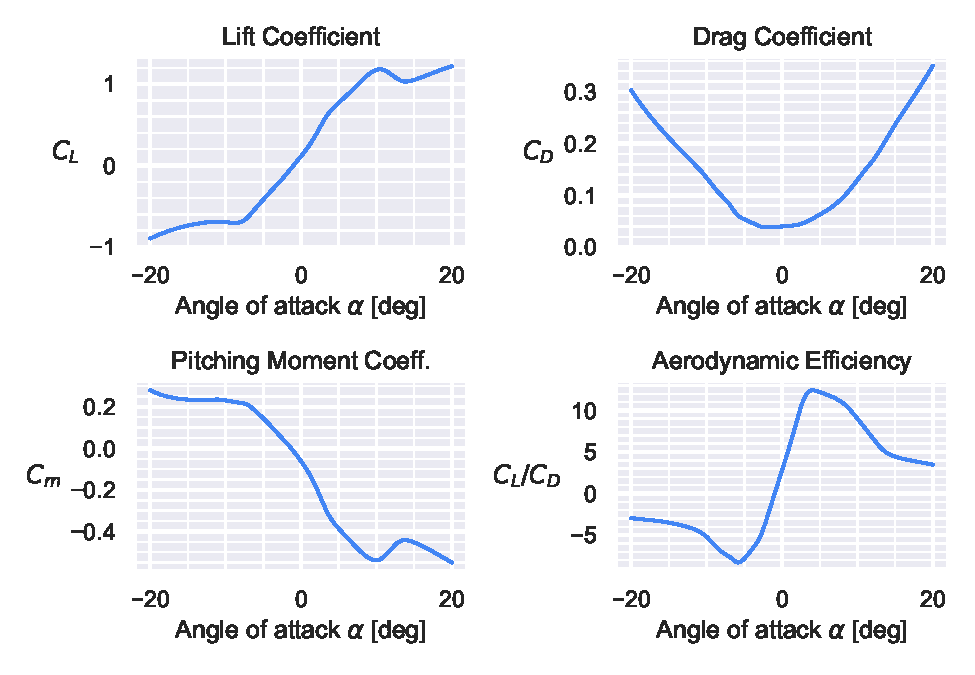
\includegraphics[width=6in]{../figures/aerobuildup_figs/polars.pdf}
    \caption{Standard static aerodynamic polars for the MIT Firefly air vehicle, computed using AeroBuildup. Analysis is an angle of attack ($\alpha$) sweep at Mach 0.15 and sea level conditions. Control surfaces are not deflected.}
    \label{fig:ab_polars}
\end{figure}

To generate the smooth plots in Figure \ref{fig:ab_polars}, 1,000 unique aerodynamic operating points were analyzed with AeroBuildup (each at a different $\alpha$). This process is benchmarked at 3.13 seconds in total on a laptop-grade CPU, or around 3 milliseconds per operating point. This is achievable due to data-level vectorization, allowing for instruction-level parallelism (SIMD) to be automatically performed. (To illustrate this, a single non-vectorized analysis takes roughly 1 second.) In either case, however, this speed combined with the ability to model viscous and compressible effects makes AeroBuildup useful for rapid aerodynamic assessment of new concepts or for aerodynamic database generation.

Figure \ref{fig:ab_polars} demonstrates that AeroBuildup captures several nuanced aerodynamic effects. For example, the lift curve captures both positive and negative stall conditions, and a lift-curve-slope nonlinearity during the attached flow regime near $\alpha=4\degree$ occurs due to sudden early upper-surface turbulent transition along the main wing. Likewise, in the moment polar, we observe a general curving-down nonlinearity, which is ultimately a consequence of the vertical displacement between the center of gravity and the neutral point. The effect of tail stall is also visible near $\alpha=13\degree$ in the moment polar, which causes a slight destabilizing effect. We also note that the moment polar shows that the vehicle requires a modest pitch-up input in order to trim at the target lift coefficient during glide ($C_L\approx 1$), which matches flight test reports by Gaubatz \cite{gaubatz_design_2024}.

\subsubsection{Stability Derivative Calculation}

AeroBuildup also supports the ability to compute stability derivatives (both static and dynamic), due to its local flow velocity computation. By default, this is computed by evaluating finite differences of the aerodynamic operating point with respect to angle of attack, sideslip, and angular rates ($\alpha, \beta, p, q, r$). This approach is the fastest strategy, because these additional analyses can be added to the vectorized evaluation enabling negligible overhead.

As an alternative to finite-differences, an interesting capability that results from the code transformations paradigm is the ability to \emph{directly} compute stability derivatives using automatic differentiation on AeroBuildup itself. Where this gets particularly unique is if this stability derivative then gets used in an optimization problem, as higher-order automatic differentiation may be required. For example, imagine we formulate an aircraft design optimization problem where the objective function is to minimize $C_{m\alpha}$. Here, we might compute $C_{m\alpha}$ by applying automatic differentiation to AeroBuildup (1 derivative). Then, we compute an exact Hessian of $C_{m\alpha}$ with respect to the design variables (2 more derivatives), to faciliate gradient-based optimization. In total, we may be performing triple-nested automatic differentiation of the original AeroBuildup analysis.

Because the operator space of the AeroSandbox numerics stack is closed under differentiation, implementing this higher-order AD is surprisingly straightforward. This fascinating capability offers unique capabilities when optimizing with respect to the evaluated gradients of an analysis, which has applications far beyond aerodynamics. Nevertheless, because AeroBuildup's implementation grants such an unusually large advantage to vectorized evaluation, simple finite-differencing is the default strategy used for stability derivative computation.

In addition to stability derivatives, other quantities of interest, like the location of the aircraft's neutral point, are computed as well. For Firefly at the Mach 0.15, sea level flight condition, AeroBuildup computes a neutral point located at $49\%$ of the main wing's root chord, or $x_{\rm np} = 241\ \rm mm$ aft of a datum placed at the vehicle's nose. For comparison, Gaubatz \cite{gaubatz_design_2024} assessed this same geometry using a vortex-lattice code (AVL \cite{avl}), which produced an estimate for the neutral point that is slightly farther aft\footnote{Note that in Gaubatz \cite{gaubatz_design_2024}, the reference datum is placed at the vehicle's tail rather than nose, so measurements must be subtracted from the vehicle length of 460 mm to convert coordinates to aircraft geometry axes with a nose datum. Note that the vehicle length of 460 mm is shorter than the bounding box of 480 mm, due to the inclusion of an external rocket igniter (briefly shown in Figure \ref{fig:firefly_conops}).}, at $x_{\rm np} = 243\ \rm mm$. Gaubatz's subsequent wind tunnel test campaign produced results\footnote{See stability derivatives reported in Table 3.2 in Gaubatz \cite{gaubatz_design_2024}.} that would indicate a neutral point at $x_{\rm np} = 236\ \rm mm$.

In any case, this indicates that the AeroBuildup result is quite consistent with both experiment and other conceptual-level aerodynamics tools. This is a particularly useful comparison, as proper computation of this neutral point reflects the fact that AeroBuildup's potential-flow-based fuselage aerodynamic computations include the destabilizing contributions of the large fuselage, which is not captured by wing aerodynamics alone.

\subsubsection{High-Angle-of-Attack Flight}

Because AeroBuildup uses sectional data that models post-stall behavior (obtained with a tool called NeuralFoil, described in Chapter \ref{chap:physics-informed-ml}), it is capable of estimating aerodynamic coefficients at extreme angles of attack and sideslip angles. This is a particularly useful capability when designing the Firefly vehicle, which must passively stabilize from a tumbling condition after deployment from the host vehicle.

For example, Figure \ref{fig:ab_high_aoa} gives a ``3D'' version of the traditional aerodynamic polars from Figure \ref{fig:ab_polars}, where these are extended to include sideslip angle $\beta$ as well as angle of attack $\alpha$, both out to $[-90\degree, +90\degree]$. In this study, the MIT Firefly air vehicle is analyzed at sea-level Mach 0.15 conditions.

Of particular interest is the ``moment flow'' diagram in the lower left of Figure \ref{fig:ab_high_aoa}, which shows how the yawing and pitching moment coefficients ($C_n$ and $C_m$) vary throughout the $\alpha, \beta$ phase space; arrows and streamlines indicate the direction that passive aerodynamic moments will tend to point the nose, from any initial vehicle orientation. This mapping is similar to a ``phase portrait'' in dynamical systems theory, though inertial effects are neglected in this strictly-static analysis. Nevertheless, this provides an excellent initial map of the vehicle's passive stability characteristics from upset flight conditions, even those well-past stall. For example, the moment flow diagram indicates that Firefly is passively stable roughly in the regime where $\beta \in [-30\degree, +30\degree]$ and for all $\alpha$, but not outside of this. This may indicate that active control inputs are required to recover from such upset conditions.

\begin{figure}[!htb]
    \centering
    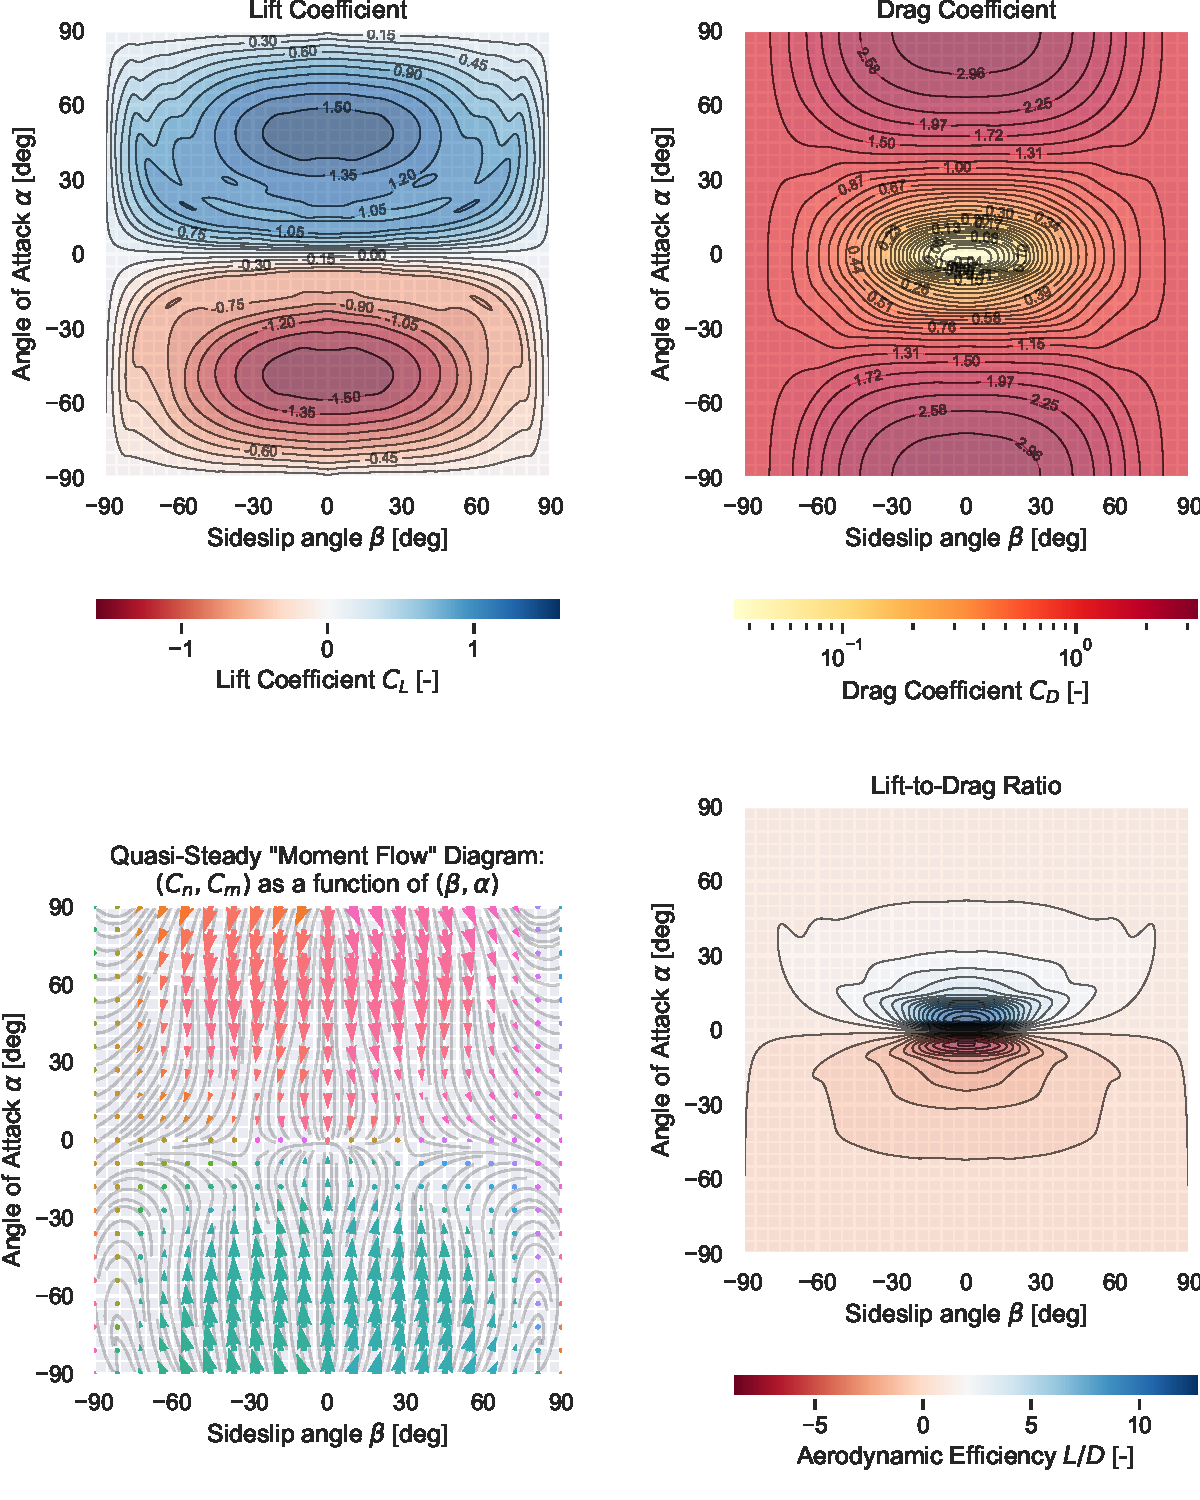
\includegraphics[width=\textwidth]{../figures/aerobuildup_figs/high_alpha.pdf}
    \caption{A ``3D'' version of standard aerodynamic polars, where lift, drag, moment (i.e., $C_n$ and $C_m$), and aerodynamic efficiency are given as a function of \emph{both} angle of attack $\alpha$ and sideslip angle $\beta$. Analysis is for the MIT Firefly air vehicle at sea-level Mach 0.15 conditions, with $\alpha$ and $\beta$ varied. Aerodynamics computed with the AeroBuildup physics model, and given for an extreme range of $\alpha, \beta \in [-90\degree, +90\degree]$ to demonstrate post-stall modeling capability. Control surfaces are undeflected in all cases.}
    \label{fig:ab_high_aoa}
\end{figure}

This kind of information about post-stall handling qualities of a candidate airframe would ordinarily not be available until well beyond the conceptual design phase. However, AeroBuildup's rapid aerodynamic analysis capability allows for this kind of analysis to be performed in a matter of seconds, enabling the designer to make informed decisions about the vehicle's passive stability characteristics early in the design process.

\subsubsection{Transonic and Low-Reynolds Flight}

Firefly uniquely operates at both low Reynolds numbers and transonic speeds, which are two flight regimes that are traditionally difficult to model with aerodynamics tools. Moreover, the \emph{combination} of these two regimes presents further challenges, as a) limited validation data is available for such conditions, and b) these two conditions create aerodynamic design drivers that are directly opposed to each other, such as the target pressure distribution in pressure recovery zones. Further details on this inherent conflict of transonic and low-Reynolds design drivers are given by Drela \cite{drela_transonic_1992}. In short, this conflict makes it challenging for a designer to know which high-level aerodynamic effects will dominate the vehicle's performance.

AeroBuildup is capable of capturing these effects simultaneously, as shown in Figure \ref{fig:ab_transonic}. Here, the MIT Firefly air vehicle is analyzed across a range of Mach numbers $M_\infty$ and angles of attack $\alpha$. In all cases, atmospheric conditions are taken at Firefly's launch altitude of 30,000 ft. Because of this, Reynolds number also changes as a function of Mach number. In these results, several notable aerodynamic phenomena are captured:

\begin{enumerate}[noitemsep]
    \item Near the zero-speed condition ($M_\infty \leq 0.05$), the Reynolds number also drops quite low, which precipitates a rise in the drag coefficient $C_D$ and a sudden reduction in the lift-curve slope $C_{L \alpha}$ as the suction-side boundary layer cannot transition.
    \item At low subsonic conditions, the expected Prandtl-Glauert-like compressibility effects on the overall pressure distribution are visible, which cause the lift curve slope $C_{L \alpha}$ to rise with increasing Mach.
    \item At transonic speeds ($M_\infty \approx 0.8$), the onset of transonic effects is clearly visible. The Mach number at which these effects begin, $\Mcr$, is a strong function of local pressure drop, and hence, angle of attack. This cross-dependency is successfully captured by AeroBuildup. After such speeds, lift drops markedly due to a buffet model, and drag rises due to the onset of wave drag. This shock effect occurs both at positive and negative angles of attack, but the wing's ability to sustain a larger pressure drop on the suction-side surface causes these transonic effects to be more pronounced at positive angles of attack.
\end{enumerate}

\noindent This provides a unique view into this combination of nuanced aerodynamic effects that is rare to obtain at the conceptual phase. Because the impact of both transonic and low-Reynolds effects can be considered together, the designer can make a meaningful prediction about which set of competing aerodynamic design drivers is likely to dominate the vehicle's performance.

\begin{figure}[!htb]
    \centering
    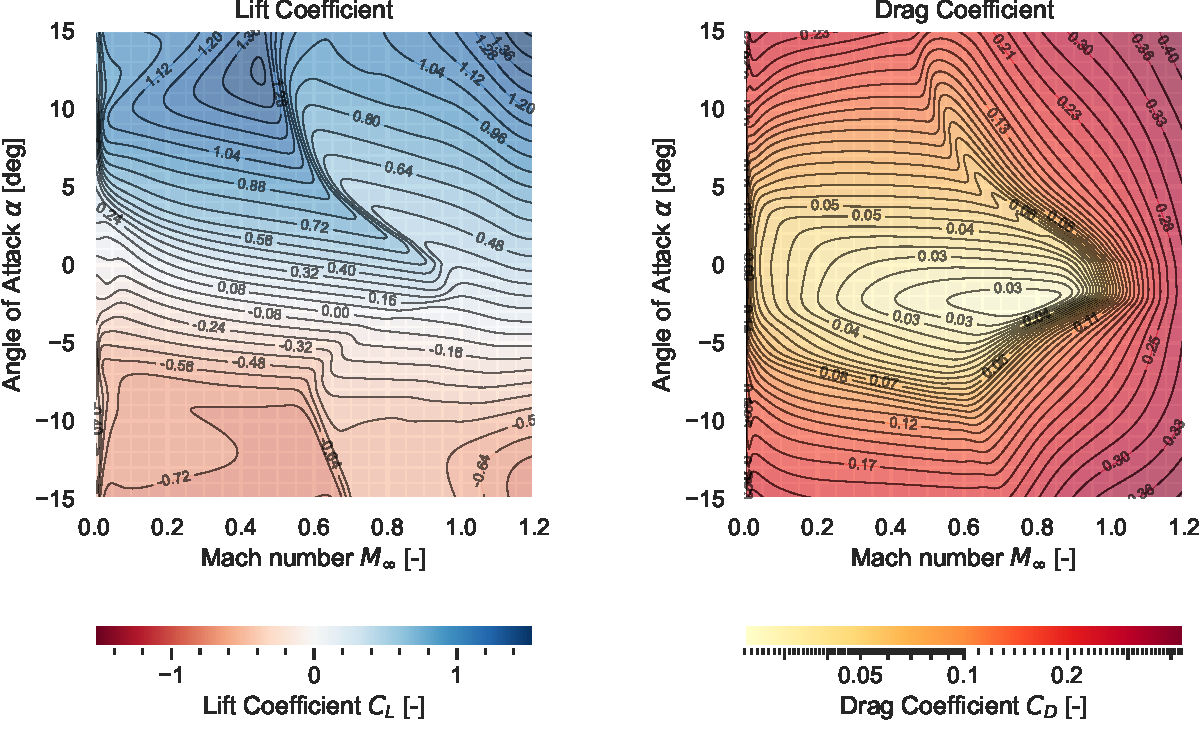
\includegraphics[width=\textwidth]{../figures/aerobuildup_figs/transonic.pdf}
    \caption{Transonic and low-Reynolds-number aerodynamic effects can be simultaneously captured by AeroBuildup. Here, the MIT Firefly air vehicle is analyzed across a range of Mach numbers $M_\infty$ and angles of attack $\alpha$. In all cases, atmospheric conditions are taken at Firefly's launch altitude of 30,000 ft. Because of this, Reynolds number also indirectly changes as a function of Mach number.}
    \label{fig:ab_transonic}
\end{figure}


% TODO use case: aerodynamic database generation to support flight simulation or time-domain testing of control laws

\section{Cross-Validation of AeroSandbox Aerodynamics Analyses}

To assess the accuracy of the three AeroSandbox aerodynamics analyses presented in Sections \ref{sec:vlm}, \ref{sec:ll}, and \ref{sec:ab}, a series of cross-validation studies were performed.

\subsection{Flying Wing Validation Study}

The first such validation study is based on a flying wing geometry described in NACA Report RM-A50K27 \cite{tinling_effects_1951}, which provides wind tunnel data as a point of comparison. This validation case study was originally organized by John Yost \cite{yost2022}, and was subsequently refined in collaboration with the author.

The geometry used in this study is described fully by Tinling and Kolk \cite{tinling_effects_1951}, and is also visualized in Figure \ref{fig:fw_geometry}. The wing has a $35\degree$ quarter-chord sweep, a span of $b=3.098\ \rm m$, an aspect ratio of $\AR = 10$, and a taper ratio of $\lambda=0.5$. A constant NACA $\mathrm{64_{1}A012}$ airfoil is used along the entire span, with no twist. The wing is analyzed at a Reynolds number of $\text{Re}=2 \times 10^6$ to match the wind tunnel conditions, corresponding to $91.3\ \rm m/s$ ($M_\infty=0.26$) at sea level.

\begin{figure}[!htb]
    \centering
    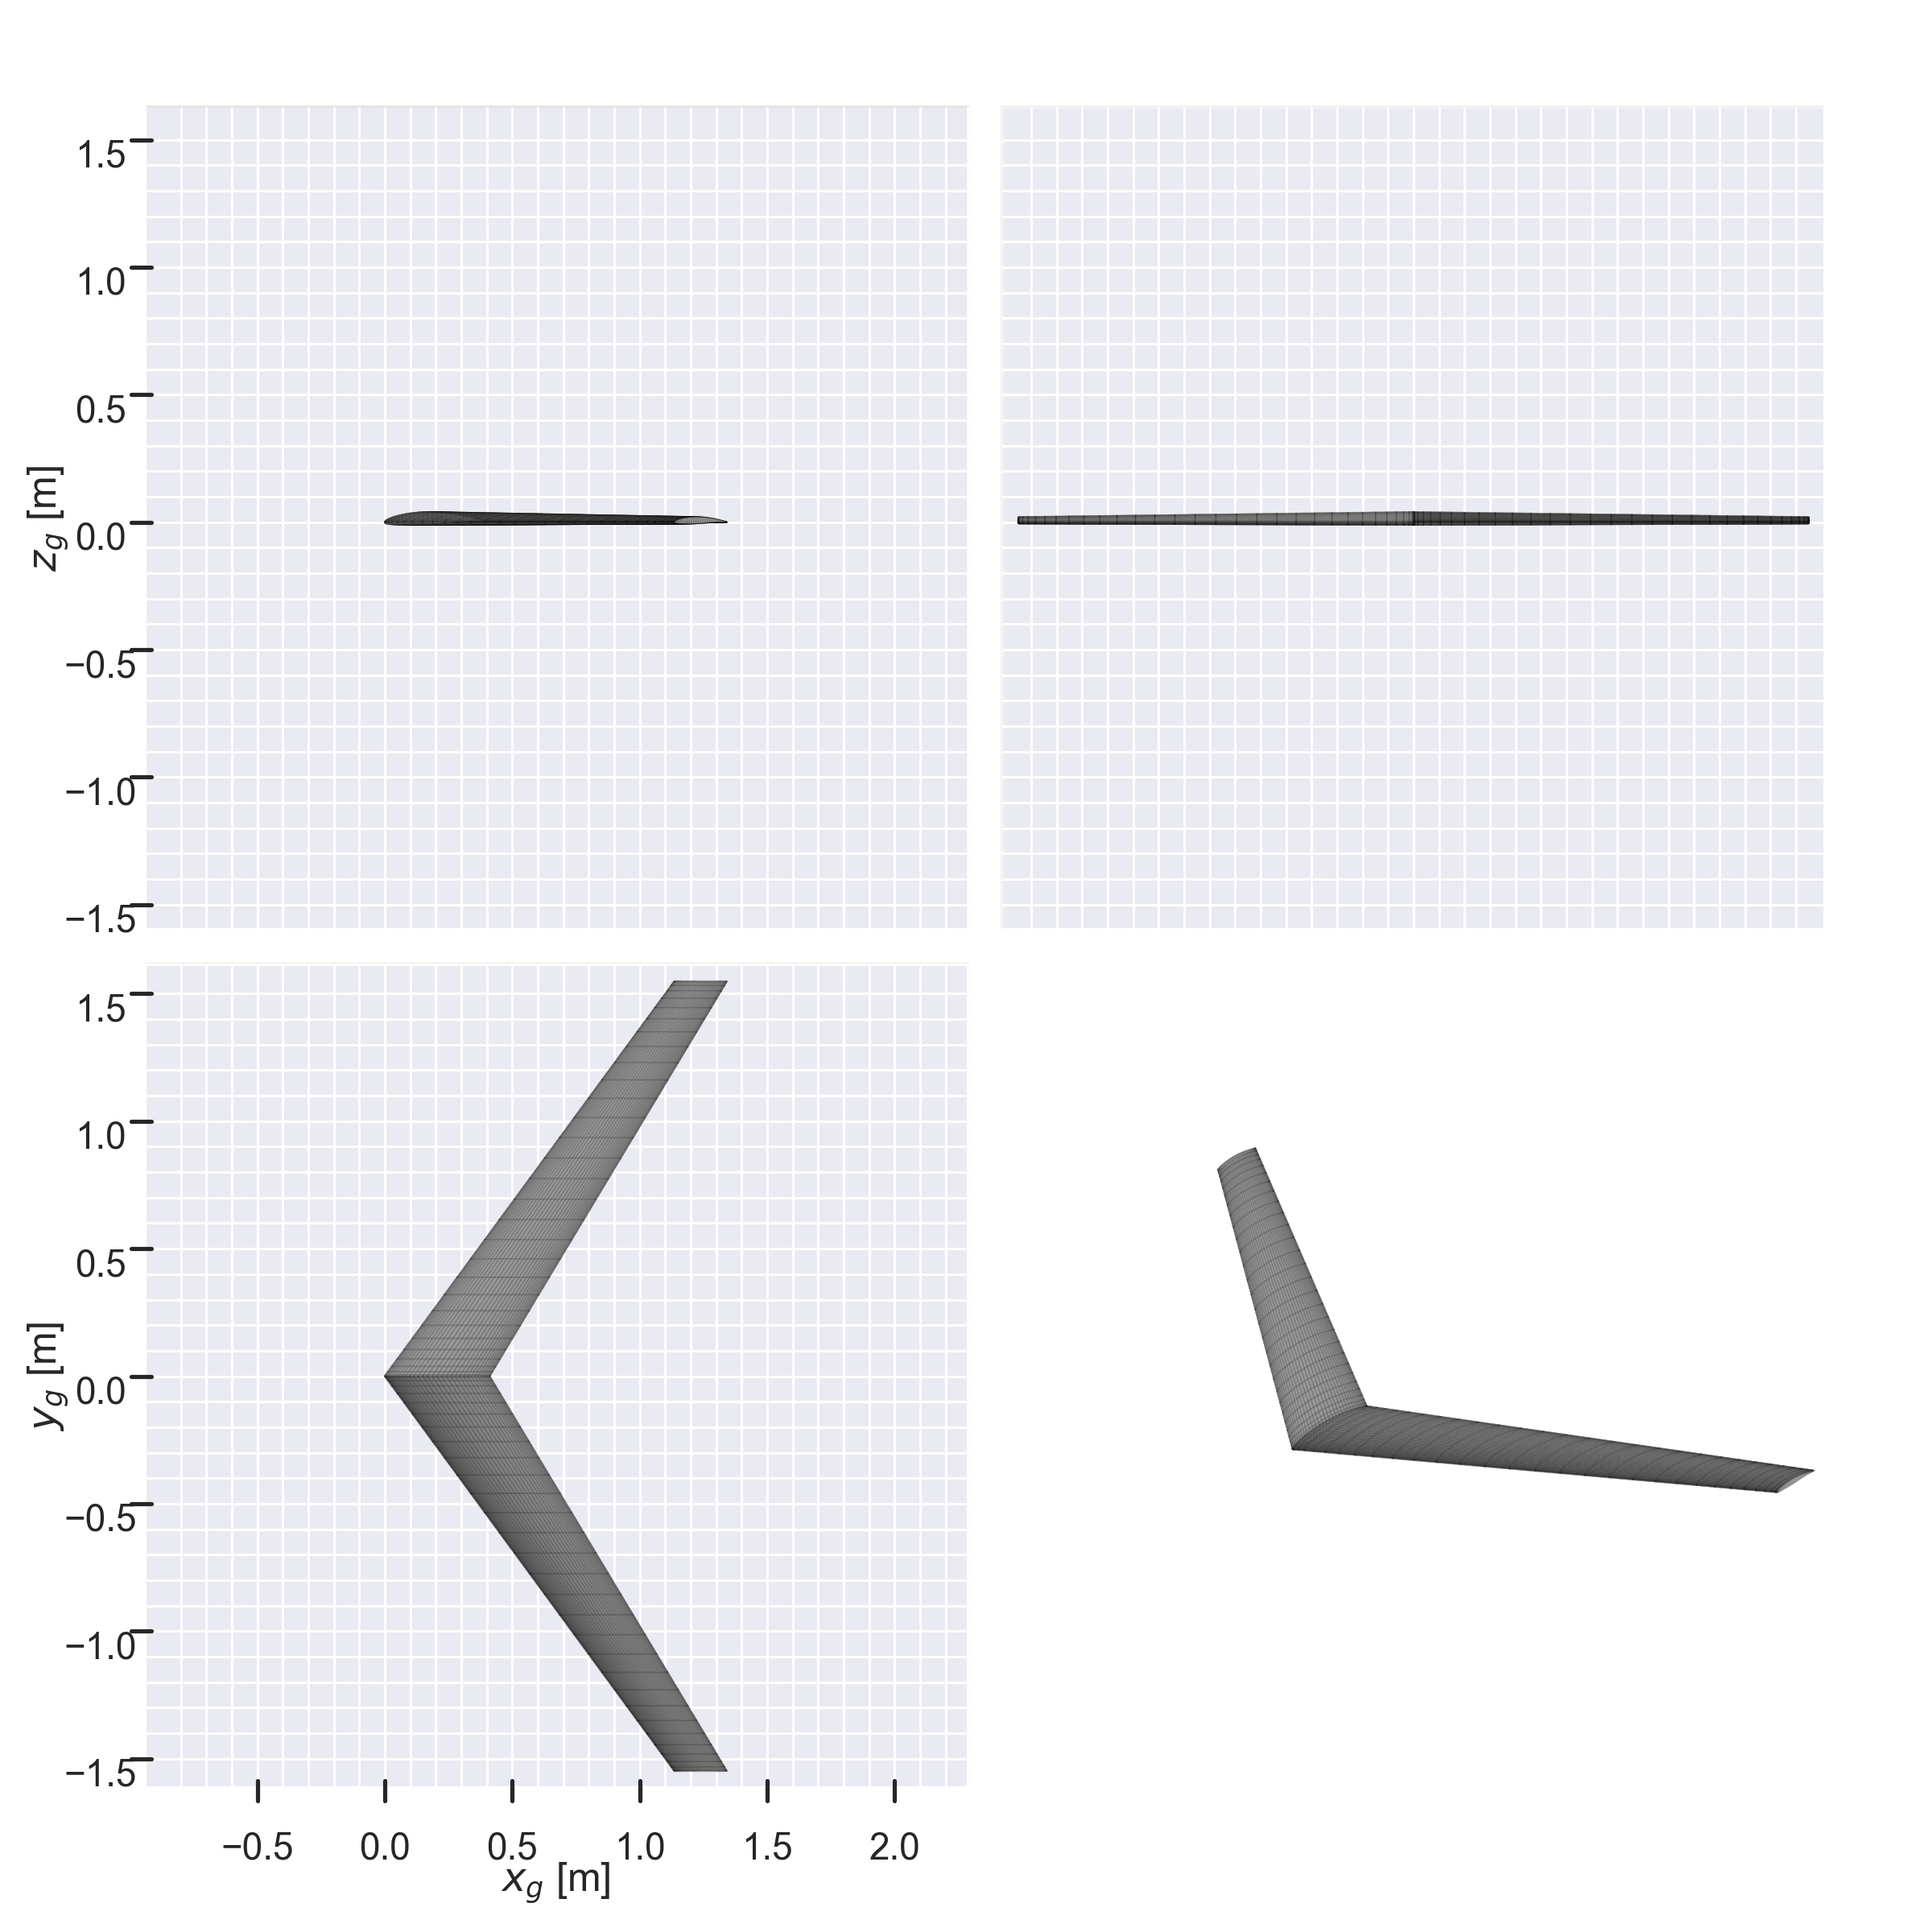
\includegraphics[width=5in]{../figures/aero_validation/flying_wing_geometry.png}
    \caption{Three-view of the flying wing aircraft geometry used in the AeroSandbox aerodynamics validation study. Based on geometry used in wind tunnel experiements in NACA Report RM-A50K27 \cite{tinling_effects_1951}.}
    \label{fig:fw_geometry}
\end{figure}

Using this geometry and freestream conditions, we perform an angle of attack sweep using the three AeroSandbox aerodynamics analyses, to compare to wind tunnel experiment. In addition, several external conceptual-level aerodynamics tools are used for comparison, including:
\begin{itemize}[noitemsep]
    \item AVL \cite{avl} (using XFoil \cite{drela_xfoil_1989} for 2D sectional data), a vortex lattice method that is widely used in conceptual aircraft design.
    \item OpenVSP's VSPAero solver \cite{mcdonald_open_2022}, which is a 3D panel method combined with form-factor-based empirical profile drag buildups.
    \item LORAAX \cite{loraax}, a fully-coupled 3D panel and 2D (strip-wise) integral boundary layer method. An iterative solution is used to obtain a force-free wake.
\end{itemize}

AVL \cite{avl} (using XFoil \cite{drela_xfoil_1989} for 2D sectional data), OpenVSP's VSPAero conceptual aerodynamics tool \cite{mcdonald_open_2022}, and Loraax, a 3D panel and integral boundary layer code. The results of this comparison are shown in Figure \ref{fig:fw_results}.

\begin{figure}[!htb]
    \centering
    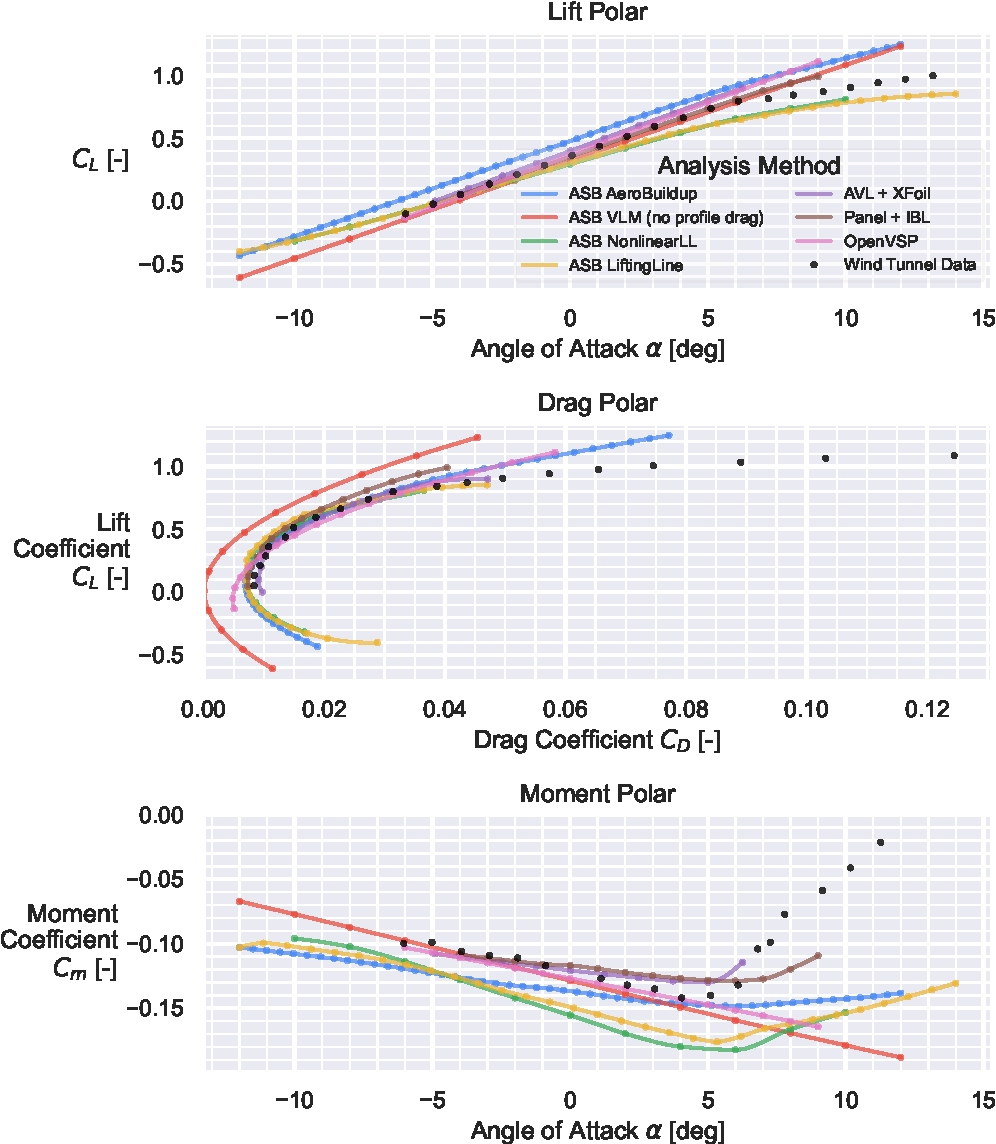
\includegraphics[width=\textwidth]{../figures/aero_validation/flying_wing_polars-crop.pdf}
    \caption{Comparison of aerodynamic polars for the flying wing geometry at $\text{Re}=2 \times 10^6$. The AeroSandbox VLM, lifting-line, and AeroBuildup analyses are compared to wind tunnel data and other conceptual-level aerodynamics tools. The wind tunnel data is reproduced from NACA Report RM-A50K27 \cite{tinling_effects_1951}.}
    \label{fig:fw_results}
\end{figure}

In the lift polar of Figure \ref{fig:fw_results}, we observe that the AeroSandbox lifting line models (both quasi-linear and fully nonlinear) capture the nonlinear $C_L(\alpha)$ dependency of the wind tunnel data quite well. Likewise, the AeroBuildup method captures the shape of the lift curve reasonably well. Interestingly, the computational lifting-line methods tend to err low on this highly-swept-wing case while the AeroBuildup method tends to err high, and for exactly opposite reasons. In reality, the lifting line of a highly-swept wing will tend to follow the geometric sweep of the wing, but it will tend to unsweep near the centerline due to the influence of the other wing half. A computational lifting-line method places the aerodynamic lifting line exactly at the locus of geometric quarter-chord-points, which then underestimates the lift at the centerline. (While there \emph{should} be a dip in the lift distribution at the centerline, a computational lifting-line method will predict a more-extreme dip than reality.) On the other hand, AeroBuildup assumes a uniform downwash\footnote{This is usually a reasonable rough assumption for low-induced-drag wings with near-elliptical lift distributions, but in a highly-swept wing case this is violated.}, which results in no dip in the lift distribution near the centerline. Of course, reality is somewhere in between these two limit cases. The ASB vortex lattice method estimates the lift quite well when flow is fully attached, but as is the case with any (linear) vortex lattice method, it struggles to capture the nonlinearities in the lift curve slope near stall.

In the drag polar of Figure \ref{fig:fw_results}, the AeroSandbox lifting line models and AeroBuildup both achieve excellent agreement with the wind tunnel data. This is notable, because this polar is chiefly responsible for overall performance prediction of the aircraft. The AeroSandbox vortex lattice method does not include any profile drag handling, and is thus not expected to match other results -- as discussed in Section \ref{sec:vlm}, the primary intended use of the VLM is for flight dynamics analysis rather than performance prediction.

In the moment polar of Figure \ref{fig:fw_results}, we see that the AeroSandbox vortex lattice method achieves very close agreement with wind tunnel data until separation occurs. This is expected, as vortex lattice methods have a long and successful history of use for conceptual stability and control analysis. The AeroSandbox lifting line methods achieve good agreement on the static stability derivative $C_{m \alpha}$, but a small constant error in the $C_m$ value itself remains. This is also likely due to underestimation of the lift at the centerline, as discussed in the lift polar. The AeroBuildup method achieves closer agreement to wind tunnel data, but it predicts a more gradual onset of stall than the sudden separation seen in experiment.

One of the notable findings of this validation study is that the quasi-linear lifting line and the fully-nonlinear lifting line yield very similar results across lift, drag, and moment polars. Because of this, the quasi-linear lifting line is recommended for use in conceptual design, as it is much faster to compute. The fully-nonlinear lifting line may be useful in specific cases with extensive and important near-stall behavior.

Nevertheless, in all cases here, the discrepancies discussed are well below the threshold of accuracy needed for conceptual aircraft design purposes. (Mostly, the deviations discussed in detail here are presented for theoretical interest.) In particular, the accurate results for the $C_D$-$C_L$ polar highlight the utility of these methods for initial aircraft performance prediction.

\subsection{Glider Validation Study}

The second validation study aims to demonstrate the relative strengths and weaknesses of the AeroSandbox aerodynamics analyses on a more complex geometry that includes multiple wings and a fuselage. This study is based on a sailplane-like geometry given in Figure \ref{fig:glider_geometry}

\begin{figure}[!htb]
    \centering
    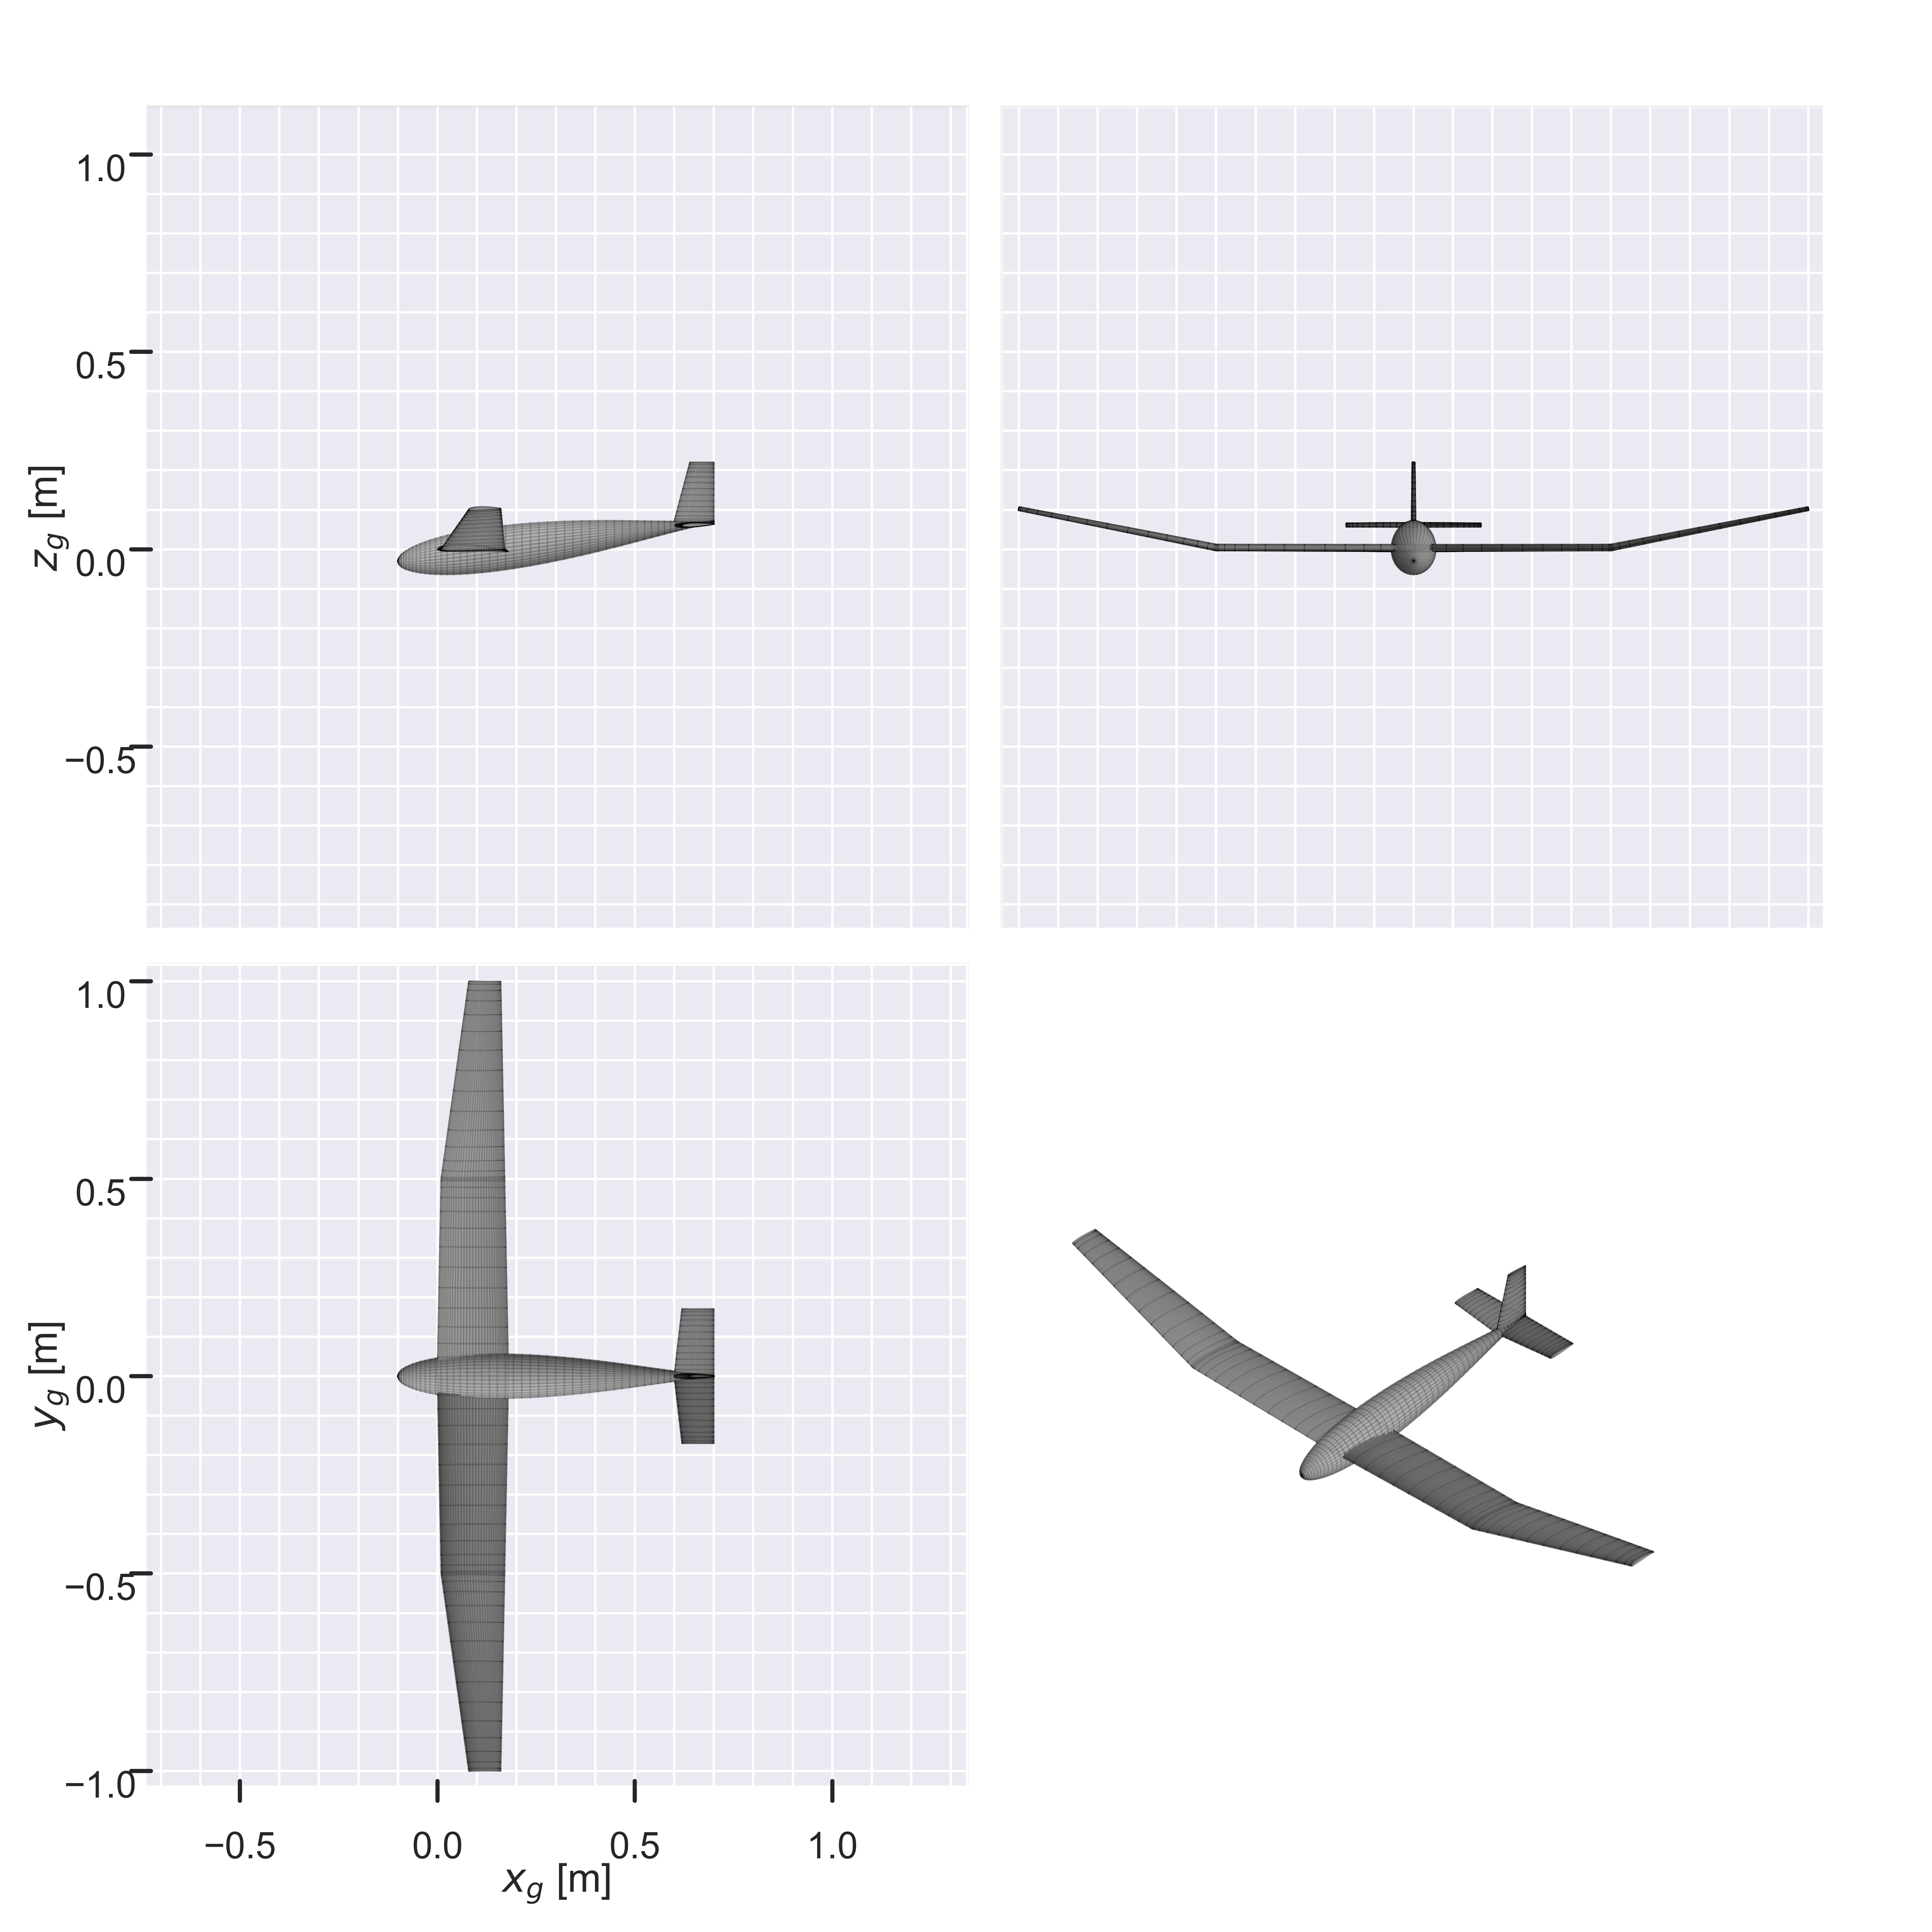
\includegraphics[width=5in]{../figures/aero_validation/glider_geometry.png}
    \caption{Three-view of the glider aircraft geometry used in the AeroSandbox aerodynamics validation study.}
    \label{fig:glider_geometry}
\end{figure}

\begin{figure}[!htb]
    \centering
    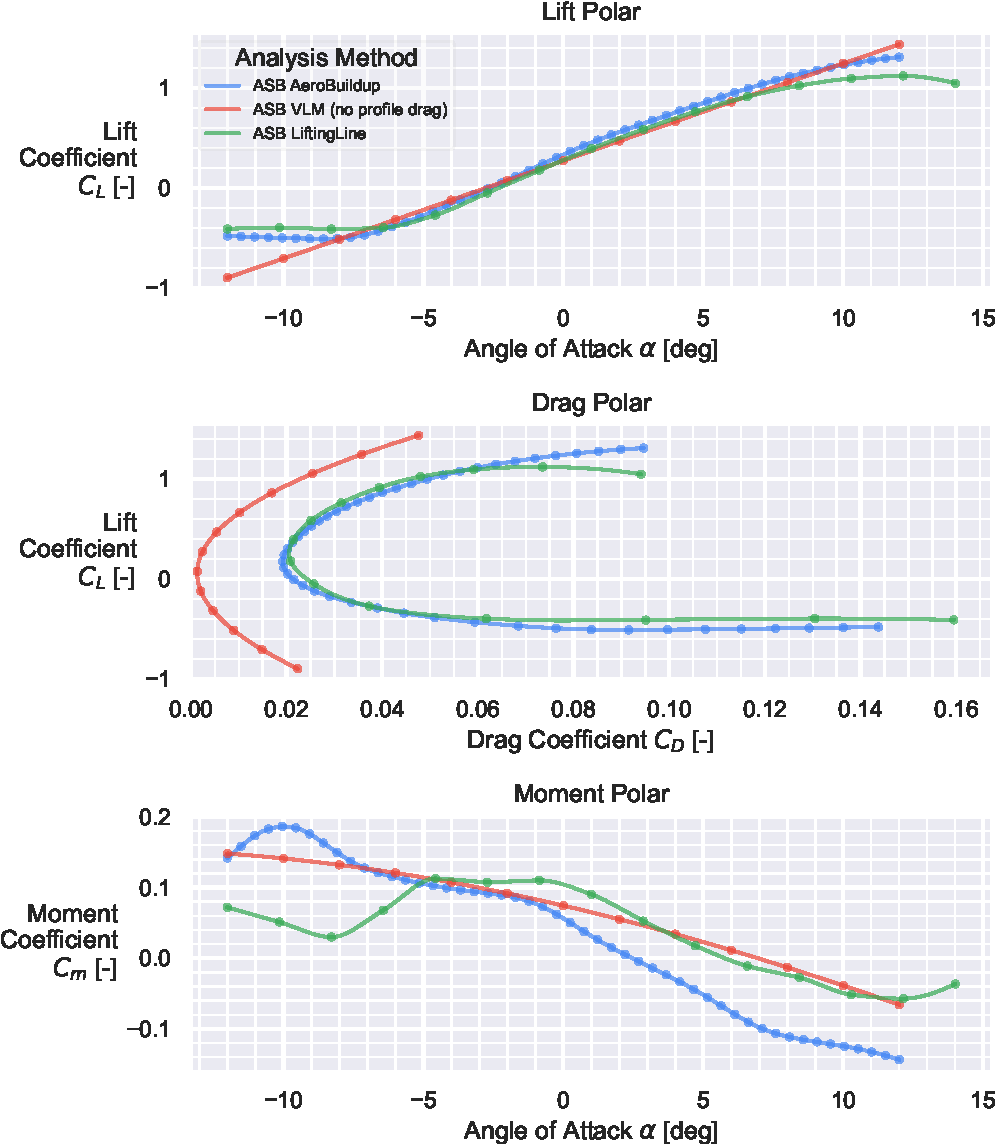
\includegraphics[width=\textwidth]{../figures/aero_validation/glider_polars-crop.pdf}
    \caption{Comparison of aerodynamic polars for the glider geometry at $\text{Re}=1 \times 10^6$. The AeroSandbox VLM, lifting-line, and AeroBuildup analyses are cross-compared to assess agreement.}
    \label{fig:glider_results}
\end{figure}


\subsection{Computational Reproducibility}

All code and geometries used in these aerodynamic validation studies are publicly available within the tutorials section of the broader AeroSandbox repository, available at \url{https://github.com/peterdsharpe/AeroSandbox/tree/master/tutorial}.


\section{Rigid-Body Equations of Motion}

%

% TODO sec:aero_validation
% TODO sec:aerobuildup